\documentclass{kursa4}

\title{Синтаксические особенности «романа в стенограмме» Е. Бочоришвили «Только
ждать и смотреть»}
\author{Матуа Ирма Отариевна}
\date{14 июня 2017 года}

\begin{document}
  \pagestyle{empty}

  \maketitle

  % \setcounter{page}{2}

  \setcounter{tocdepth}{2}
  \renewcommand\contentsname{}
  \tableofcontents

  \pagestyle{plain}

  \chapter{Введение}

    Исследователи современной художественной литературы отмечают
    тенденцию к появлению новых жанровых образований. В частности, М. Ю.
    Звягина пишет:

    «Авторские жанровые формы стали важной составляющей современной
    жанровой системы. Наблюдения показывают, что с периферии они
    переместились в центр эпической системы жанров. Тенденция к игре с
    жанром, попытки так или иначе трансформировать традиционные жанры,
    создание их модификаций~--- все это отличительные черты не только
    эстетики постмодерна и авангарда, но и приемы, ставшие привычными для
    реализма. Актуализация приема трансформации жанров во всех основных
    художественных методах освоения мира и позволила авторским жанровым
    формам занять если не доминирующее, то одно из центральных мест в
    современной жанровой
    системе».\footnote{\textit{{Звягина М. Ю.
    }}{Жанровые трансформации в русской прозе второй
    половины 20~--- нач. 21 века. Астрахань, 2016. С.28}}

    Новый и непривычный, авторский жанр формулирует для читателя
    определенную установку на прочтение. В случае, если жанр имеет
    составное поименование (к примеру, «роман-мистерия», «роман-житие»),
    читателю необходимо отыскивать в произведении особенности указанных в
    названии компонентов и в соответствии с этим прочитывать текст. На
    такое стремление автора дать определенный ключ к восприятию текста
    указывает Т. Маркова:\newline
    «Жанровый подзаголовок создает у читателя определенные ожидания
    содержания и формы текста. Таким способом автор активизирует
    читательское восприятие за счет ассоциативной разветвленности,
    необходимости одновременного учета разных составляющих. С другой
    стороны, авторский подзаголовок вступает в диалогические (а иногда и
    оппозиционные) отношения с жанровым каноном, национальной традицией,
    сигнализируя об экспериментальном характере
    произведения».\footnote{{
    }\textit{{Маркова Т. }}{Авторские
    жанровые номинации в современной русской прозе как показатель кризиса
    жанрового сознания// Вопросы литературы. 2001. №1. }}

    По справедливому замечанию Т. Марковой, одновременно автор вступает
    в диалог и с традиционной, канонической формой, на теле которой
    происходят изменения. 

    Елена Бочоришвили~--- канадский русскоязычный писатель грузинского
    происхождения,~--- является автором двух сборников, изданных в 2012 и
    2015 годах, которые состоят из небольших текстов, по размерам
    сопоставимых с повестью или рассказом. Однако Е. Бочоришвили жанр
    текстов определяет как \textit{roman stenographique}, или
    «\textit{роман в стенограмме}». 

    {Стенограмма~--- текст, представляющий дословную
    запись устной речи по методу
    стенографии.}\footnote{{Российский энциклопедический
    словарь/Гл. ред. А. М. Прохоров. М., 2001 }\par
    {Ссылка на электронный ресурс:
    https://clck.ru/AuxNo}}

    {Стенография}\textbf{{ }}(от греч.
    στενός~--- узкий, тесный и γράφω~--- пишу)~--- скоростное письмо, основанное
    на применении специальных систем знаков и сокращений слов и
    словосочетаний, позволяющее вести синхронную запись устной речи и
    рационализировать технику письма. Скорость стенографического письма
    превосходит скорость обычного в 4-7
    раз.\footnote{{Большая советская энциклопедия /Сл.
    cтатья: Соколов Н. Н., Скородумова Н. П.~--- М., 3 изд. 1970~--- 1978Ссылка
    на электронный ресурс: https://slovar.cc/enc/bse/2044790.html}}

    Важное для нас толкование определения «стенографический» находим в Новом
    словаре иностранных слов{: }1) записанный по способу
    стенографии; 2) \textit{перен.} \textbf{совершенно точный,
    буквальный}\footnote{\textit{{Нечаева И. В., Захаренко
    Е. Н., Комарова Л. Н. }}{Новый словарь иностранных
    слов.~--- М., 2008. Ссылка на электронный ресурс:
    https://slovar.cc/rus/inostr-nov/1431100.html}}. 

    Из приведенных определений следует, что при создании стенограммы: 1)
    используются знаки и сокращения вместо полной формы; 2) дословно
    фиксируется устная речь. Цель данного метода можно сформулировать таким
    образом: максимальная рационализация способа письма, которая
    заключается в \textbf{сохранении всего содержания сказанной речи при
    использовании наиболее краткой формы выражения этого содержания.} 

    Очевидно, что текст стенограммы не является художественным
    осмыслением реальности. Напротив, он являет собой максимально
    беспристрастное ее отражение. Личность стенографа исключена из
    стенографических записей. 

    Ориентация на стенографическую запись приводит автора к
    необходимости выбирать языковые средства, соответствующие принципам
    стенограммы. Как отмечают исследователи, создание новых форм в
    современном прозаическом тексте производится, в первую очередь, путем
    работы с синтаксической структурой произведения. 

    {«Сегодня одновременное упрощение (аналитическая
    дробность) и усложнение синтаксиса (создаваемое, в частности,
    комплексным использованием новых явлений), выступает на передний план
    как специальная забота
    автора».}\footnote{\textit{{Мартьянова И. А.
    }}{Функционирование синтаксических единиц в
    современной русской прозе// Вестник Череповецкого государственного
    университета. Выпуск № 2 (37) / том 1 / 2012. С.82}}

    {Культуролог В. П. Руднев, характеризуя язык прозы,
    отводит синтаксису основополагающую роль в формировании новых принципов
    построения текста: «Если поэзию действительно можно назвать
    искусством слова, то проза скорее~--- это искусство предложения. Слово
    более гибко, поэтому философия слова на протяжении века изменялась
    много раз: своя концепция слова была у символизма, своя~--- у акмеизма,
    конструктивизма, обэриутов, концептуализма. Философия предложения
    фундаментально изменилась в ХХ в. только один раз~--- при переходе от
    логического позитивизма к зрелой аналитической философии.
    \textless{}...\textgreater{} Обновление языка в модернистской прозе
    происходит прежде всего за счет обновления и работы над
    синтаксическими конструкциями; не над словом, а над
    предложением».}\footnote{\textit{{ Руднев В. П.
    }}{Словарь культуры XX века. М.,1997. С.238—240 }}

    {Таким образом, целью данного исследования является
    выявление синтаксических особенностей «романов в стенограмме» Е.
    Бочоришвили.}

    {Задачи исследования:}
    % \liststyleWWNumxiii
    \begin{enumerate}
      \item Теоретическое описание жанра стенограммы и
      основных синтаксических категорий, связанных с реализацией принципов
      стенограммы в художественном тексте;
      \item Поиск синтаксических средств, позволяющих
      воспроизвести основные принципы стенограммы в исследуемых
      художественных текстах;
      \item Описание функций синтаксических средств, не
      отвечающих задачам стенографического письма.
    \end{enumerate}

    \textbf{Объектом} данного исследования являются «романы в
    стенограмме» как пример современной жанровой трансформации. Источником
    послужили тексты Елены Бочоришвили «Опера» и «Мои душистые старички и
    благоухающие старушки», входящие в состав сборника «Только ждать и
    смотреть»\footnote{{
    }\textit{{Бочоришвили Е.}}{Только
    ждать и смотреть// изд. Corpus. М., 2015}}. 

  \setcounter{chapter}{0}
  \chapter {Глава 1. Особенности стенограммы и
  синтаксические способы их имитации в художественном тексте.}
  % \setcounter{chapter}{1}

    \section {Характеристика стенограммы. Фиксация
    речи, описание обстановки, точка зрения пишущего.}

      Жанр произведений Е. Бочоришвили определяется как сложный, состоящий
      из нескольких жанров: романа и стенограммы. Для того, чтобы выявить
      основные черты этого комбинированного жанра, необходимо понять, что
      именно будет заимствоваться из стенограммы и получать свое отражение в
      художественном тексте. Очевидно, заимствуется цель стенограммы и
      основные принципы, непосредственно следующие из этой цели, а не методы:
      использование специальных знаков и сокращений (текст Е. Бочоришвили
      состоит из знаков привычной нам языковой системы). 

      Современное понимание стенографии и основных ее принципов будет
      более полным, если обратиться к истории явления:

      {В журнале «Современник» 1958 г. в рецензии на
      книгу М. Иванина}\footnote{{
      }\textit{{Иванин М. И. }}{О
      стенографии или искусстве скорописи и применении её к русскому языку.
      Спб., 1858}}{ находим: «Главное назначение стенографии
      то, что посредством ея можно дословно записывать речи говорящего.
      Поэтому она имеет наибольшее применение там, где процветает ораторское
      красноречие, где существуют публичные суды и торжественные совещания в
      делах политических, одним словом, где существует
      гласность...».}\footnote{{ Цит. по:
      }\textit{{Юрковский А. М.
      }}{Стенография сквозь века. М., 1969.
      С.55}}{ }

       Приведенное определение стенографии, наряду с бытующими в
      современных словарях, рассмотренных в главе «Введение» данной работы,
      свидетельствует о том, что стенография дает возможность дословно
      зафиксировать устную речь. Кроме того, определение снабжено
      информацией о типичных сферах функционирования данного способа
      письма, отличительной чертой которых является гласность. 

      В тексте стенограммы содержится точное указание на: время, в которое
      происходит событие; авторов реплик. Кроме того, действия участников
      события могут комментироваться стенографом, если они имеют значение для
      события. Комментарии эти лаконичны, для них характерны простота и
      ясность изложения (пр. \textit{аплодисменты}). Примеры текстов
      стенограммы приведены в Приложении к данной работе. 

      Задача стенографа~--- наиболее точно и без изменений зафиксировать
      факты, в точности отразить речь говорящих, не привнося в запись
      собственную оценку событий. В стенограмме отражен синтаксис,
      характерный для речи говорящего, а не общее содержание речи,
      лексическое наполнение фразы, приведенное в соответствие с тем или иным
      стилем. 

    \section{Категория «образ автора» и способы
    имитации безоценочности.}

      Стенограф как создатель стенограммы не реализует свою оценку по
      отношению к фиксируемым событиям. Необходимо понять, как создатель
      художественного произведения являет себя в тексте, имитирующем
      стенограмму, и по отношению к кому можно говорить о наличии или
      отсутствии оценки описываемых событий. 

      Понятие «образ автора» неразрывно связано с именем В. В.
      Виноградова, который произвел многомерный филологический анализ
      «Пиковой дамы» А. С. Пушкина и показал, что осмысление структуры
      повествования дает ключ к пониманию произведения:

      «Символы, характеры и стили литературы осложняются и преобразуются
      формами воспроизводимой действительности. В сферу этой изображаемой
      действительности вмещается и сам субъект повествования~--- «образ
      автора». Он является формой сложных и противоречивых соотношений между
      авторской интенцией, между фантазируемой личностью писателя и ликами
      персонажей. В понимании всех оттенков этой многозначной и многоликой
      структуры образа автора~--- ключ к композиции целого, к единству
      художественно-повествовательной системы
      Пушкина».\footnote{\textit{{Виноградов В. В.
      }}{«Стиль «Пиковой дамы» // Временник Пушкинской
      комиссии, т. 2, 1936. С.75—86.}} 

      Так, «образ автора» является внутритекстовой категорией, важнейшей
      для интерпретации языковых единиц текста, а также для конструирования
      языковой личности автора.\footnote{{Термин «языковая
      личность» используется в значении: «Личность, выраженная в языке
      (текстах) и через язык; личность, реконструированная в основных своих
      чертах на базе языковых средств». }\textit{{Караулов
      Ю.Н. }}{Русский язык и языковая личность. М., 1987.
      С.38}} 

      Современные исследователи языка нарратива, такие как Е. В.
      Падучева\footnote{\textit{{Падучева Е. В.
      }}{Семантические исследования. Семантика времени и
      вида в русском языке. Семантика нарратива.~--- М.: Языки славянской
      культуры, 1996. Изд. 2-е, 2010. С.201—202[далее в сносках: Указ. соч.
      1.]}}, развили идеи В. В. Виноградова, уточнив, однако,
      нетождественность создателя текста (к примеру, А. С. Пушкина) тому
      субъекту повествования, который эксплицитно представлен в
      тексте:\newline
      «О б р а з автора, а точнее сказать~--- п о в е с т в о в а т е л ь :
      именно повествователь является тем субъектом сознания, который
      непосредственно воплощен в тексте и с которым имеет дело читатель». 

      В. И. Заика, соглашаясь с Е. В. Падучевой, определяет художественное
      произведение как реализованную автором художественную модель, частью
      которой и является повествователь:

      «Разведение автора и повествователя~--- условие лингвистического
      анализа художественного текста. Моделируя признаки повествующего лица,
      лингвист не говорит о реальном авторе. Обнаружение, расшифровка
      признаков (мировоззрения, склонностей, болезней, пороков и под.) автора
      (как реальной личности) в тех или иных элементах художественной модели
     ~--- прерогатива критика, литературоведа. Имманентный (по В.В.
      Виноградову) анализ текста, осуществляемый лингвистом, предполагает
      характеристику субъекта повествования как компонента художественной
      модели».\footnote{\textit{{Заика В. И.
      }}{Повествователь как компонент художественной модели
      //Говорящий и слушающий: Языковая личность, текст, проблемы обучения.
      СПб, 2001. C.384}}

      «Смерть автора», зафиксированная Р. Бартом еще в 1967г., определила
      фокус современной лингвистики нарратива:\newline
      «С точки зрения лингвистики, автор есть всего лишь тот, кто пишет,
      так же как «я» всего лишь тот, кто говорит «я»; язык знает «субъекта»,
      но не «личность», и этого субъекта, определяемого внутри речевого акта
      и ничего не содержащего вне его, хватает, чтобы «вместить» в себя весь
      язык, чтобы исчерпать все его
      возможности».\footnote{\textit{{Барт
      Р.}}{ Избранные работы: Семиотика. Поэтика. М., 1994.
      С.387}}

      Однако текст, совмещая в себе авторский замысел и значение
      конкретных составляющих его единиц языка, «представляет собой
      завершенную с точки зрения его создателя, но в смысловом и
      интенциональном плане открытую для множественных интерпретаций линейную
      последовательность языковых знаков, выраженных графическим (письменным)
      или звуковым (устным) способом, семантико-смысловое взаимодействие
      которых создает некое композиционное единство, поддерживаемое
      лексико-грамматическими отношениями между отдельными элементами
      возникшей таким образом
      структуры»\footnote{\textit{{Гончарова Е. А., Шишкина
      И. П. }}{Интерпретация текста. Немецкий язык. М.,
      Высшая школа, 2005. 368 с. }}.

      Н. С. Валгина, суммируя семантический и формальный подход к изучению
      единиц текста, отмечает: «Как ни важно изучение речевой организации
      текста (выявление основных единиц текста, способов изложения), это
      изучение не может оказаться полным и адекватным, если оставить без
      внимания такое важное для текстообразования и текстовосприятия понятие,
      как авторская модальность, скрепляющая все единицы текста в единое
      смысловое и структурное целое. \textless{}...\textgreater{} Модальность
      текста~--- это выражение в тексте отношения автора к сообщаемому, его
      концепции, точки зрения, позиции, его ценностных ориентации,
      сформулированных ради сообщения их читателю. Эта авторская оценка
      изображаемого всегда связана с поиском адекватных способов выражения.
      Способы выражения этого отношения и оценки могут быть различными,
      избирательными для каждого автора и разновидности текста, они
      мотивированы и целенаправлены. Над выбором этих способов всегда, таким
      образом, стоит какая-то неречевая задача, реализация которой и создает
      свою модальность текста».\footnote{\textit{{Валгина Н.
      С. }}{Авторская модальность. Образ автора // Теория
      текста. М., 2004. С.96—97}} 

      Итак, для понимания модальности текста необходим анализ языковых
      единиц в аспекте их функционирования в конкретном произведении и
      подчиненности общему замыслу. «{Текстовая модальность,
      таким образом, выявляется тогда, когда читатель в состоянии составить
      себе представление о каком-то тематическом поле, т. е. о группе
      эпитетов, сравнений, описательных оборотов, косвенных характеристик,
      объединенных одной доминантой и разбросанных по всему тексту или по его
      законченной части».}\footnote{\textit{{Гальперин И. Р.
      }}{Текст как объект лингвистического исследования. М,
      2006. С.117}}{ }

      В тексте реализуется и модальность более низкого порядка:
      «Модальность на уровне предложения-высказывания достаточно изучена и
      определяется обычно как категория, выражающая отношение говорящего к
      содержанию высказывания (субъективная модальность) и отношение
      последнего к действительности (объективная модальность). В первом
      случае модальность создается специфическими модальными словами,
      частицами, междометиями (к счастью, к сожалению, увы, ведь и др.); во
      втором случае модальность создается прежде всего формами наклонения
      глаголов и словами, выражающими значение утверждения, возможности,
      пожелания, приказания и др. \textless{}...\textgreater{}Таким образом,
      модальность реализуется на лексическом, грамматическом и интонационном
      уровне».\footnote{\textit{{Валгина Н. С.
      }}{Авторская модальность. Образ автора // Теория
      текста. М., 2004. С.96}} 

      Далее, необходимо остановиться на том, в чем отличие повествователя
      как элемента художественного мира от «вненаходимого» автора в аспекте
      их участия в коммуникативной ситуации и описать элементы,
      сигнализирующие о присутствии субъекта сознания, так или иначе
      выражающего свое отношение к содержанию высказывания. 

      К концу XX в. обозначилась тенденция к коммуникативному подходу в
      изучении языка. Г. А. Золотова определяет текст как «средство общения,
      то, ради чего существует язык и и все его элементы как части
      целого».\footnote{\textit{{Золотова Г. А.
      }}{О традициях и тенденциях в современной
      грамматической науке//Синтаксис современного русского языка.
      Хрестоматия с заданиями. СПб, 2013. С.31}} Так, текст рассматривается в
      качестве компонента речевой ситуации. \newline
      Е. В. Падучева выделяет следующие признаки канонической речевой
      ситуации: 

      % \liststyleWWNumxiv
      \begin{enumerate}
      \item Высказывание имеет Говорящего и Адресата~--- конкретно-референтного
      (а не обобщенного, как, например, «мой читатель» в «Онегине») и не
      совпадающего с самим говорящим. 
      \item Момент создания высказывания Говорящим совпадает с моментом его
      восприятия Адресатом, т. е. Адресат~--- это Слушающий. 
      \item Говорящий и Адресат находятся в одном и том же месте и имеют общее
      поле зрения. 
      \end{enumerate}
      Обязательное «нулевое» условие (единство мира): тождество мира
      коммуникантов и мира их референции.\footnote{\textit{{
      Падучева Е. В. }}{В. В. Виноградов и наука о языке
      художественной прозы // Известия РАН. Серия литературы и языка. Т. 54,
      № 3, 1995. С.43 [далее в сносках: Указ. соч. 2]}} 

      Анализируя коммуникавную ситуацию нарратива, Е. В. Падучева
      обнаруживет в ней полное несоблюдение условий канонической речевой
      ситуации (исключая мемуары, в которых соблюдается хотя бы нулевое
      условие): «Автор отделен от своего высказывания. Читатель имеет дело
      только с текстом, а с его создателем~--- лишь постольку, поскольку тот
      отразился в тексте. \textless{}...\textgreater{} Другая причина~---
      вымысел. Автор художественного текста создает вымышленный мир, который
      выдается к~а~к \ б~ы за фрагмент реального. В разговорном дискурсе
      говорящий сам принадлежит тому реальному миру, о котором он говорит;
      между тем автор художественного текста сам не принадлежит миру
      создаваемого им текста».\footnote{\textit{{ Падучева
      Е. В. }}{Указ. соч. 1. С.200—201}} \newline
       Затем исследователь делает вывод о том, что не все существенные
      единицы разговорного языка могут быть употреблены в нарративе, по
      крайней мере без изменения значения: «Поскольку изменение интерпретации
      происходит под влиянием изменившейся коммуникативной ситуации,
      затронуты в первую очередь должны быть те языковые элементы, семантика
      которых в принципе связана с коммуникацией. Это те элементы языка,
      которые мы будем далее называть э~г~о~ц~е~н~т~р~и~ч~е~с~к~и~м~и~--- слова
      и конструкции, содержащие отсылку к говорящему
      (ego)».\footnote{\textit{{ Падучева Е. В.
      }}{Указ. соч. 1. С.201}} 

      Эгоцентрические элементы языка, в зависимости от их ориентации на
      каноническую или неканоническую речевую ситуацию, делятся на первичные
      и вторичные соответственно.\footnote{\textit{{
      Падучева Е. В. }}{Указ. соч. 2. См.: С.44}} 

      Первичные эгоцентрики:

      % \liststyleWWNumi
      \begin{enumerate}
        \item Дейктические слова и элементы (местоимения я, ты, здесь, сейчас,
        тут, там, этот, тот или русские частицы вон и вот)
        \item Показатели так называемой {с~у~б~ъ~е~к~т~и~в~н~о~й} \ {м~о~д~а~л~ь~н~о~с~т~и}~--- вводные слова; предложения с эксплицированной иллокутивной
        функцией; модальные слова и частицы, которые подразумевают говорящего,
        и т. п.
      \end{enumerate}

      Синтаксическая неподчинимость является общим свойством для первичных
      эгоцентриков и может использоваться как синтаксический тест для
      выявления первичной
      эгоцентричности.\footnote{\textit{{ Падучева Е. В.
      }}{Указ. соч. 1. См.: С.298—299}} Под синтаксической
      неподчинимостью понимается возможность употребление слова или
      конструкции «только в синтаксически независимой позиции, т. е. в
      составе главного предложения, а постановка предложения с таким словом
      или конструкцией в позицию придаточного приводит к
      аномалии».\footnote{\textit{{ Падучева Е. В.
      }}{Указ. соч. 1. С.297}} Заметим, что под «главным»
      предложением понимается «предложение, которому соответствует отдельный
      речевой акт. В самом деле, есть придаточные, в составе которых многие
      типы синтаксически неподчинимых предложений допустимы: это, например,
      придаточные с постопозитивно употребленными союзами \textit{поскольку,
      потому что, хотя} или с аппозитивным
      \textit{который}».\footnote{\textit{{ Падучева Е. В.
      }}{Указ. соч. 1. С.299}}

      Первичные эгоцентрики ориентированы на говорящего в канонической
      речевой ситуации. У говорящего Е. В. Падучева выделяет следующие
      роли:\footnote{\textit{{ Падучева Е. В.
      }}{Указ. соч. 1. С.262—265}}

      \liststyleWWNumiii
      \begin{enumerate}

        \item Говорящий как субъект дейксиса; \newline
        Обнаруживает себя через эгоцентрики с семантикой пространственного и
        временного расположения. 

        \item Говорящий как субъект речи; \newline
        Его найдем в высказываниях с иллокутивной функцией, в обращениях, а
        также поименованиях «себя~--- другого» через местоимения «я~--- ты».

        \item Говорящий как субъект сознания; \newline
        Является подразумеваемым субъектом «в контексте слов и синтаксических
        конструкций, где субъект ментального, эмоционального или волитивного
        состояния подразумевается семантикой предиката, но не выражен или даже
        не может быть выражен в тексте высказывания; такое состояние обычно
        интерпретируется как состояние говорящего». 

        \item Говорящий как субъект восприятия.
       
      \end{enumerate}

      \bigskip

      Как видим, для осуществления 1 и 4 ролей говорящего необходима
      физическая воплощенность повествователя. 

      Для того, чтобы показать, каков должен быть повествователь, более
      всего совпадающий с «каноничным», коротко изложим основные понятия,
      используемые в типологии повествовательных форм Е. В.
      Падучевой.\footnote{\textit{{ Падучева Е. В.
      }}{Указ. соч. 1. С.203—204}} \newline

      Повествовательные формы:
      % \liststyleWWNumvi
      \begin{enumerate}
        \item Старозаветный нарратив. Повествование от 1 лица; перволичный
        повествователь, рассказчик; 
        \item Традиционный нарратив. Повествование от 3 лица; аукториальный
        повествователь;
        \item Свободно-косвенный дискурс (СКД). «Повествователь (экзегетический)
        частично уступает персонажу свое право на речевой акт. Возникает чисто
        литературная фигура~--- говорящий в 3-м лице,~--- невозможная в разговорном
        языке».
      \end{enumerate}

      В зависимости от степени причастности миру текста:
      \begin{enumerate}
        \item Повествователь, являющийся частью описываемого мира,
        совершающий поступки, имеющий биографию~--- диегетический. 
        \item Повествователь неперсонифицированный~--- экзегетический. 
       \end{enumerate} 

      Благодаря схожести перволичного диегетического повествователя с
      каноническим говорящим (рассказчик может выполнять все четыре роли
      говорящего) все первичные эгоцентрические элементы языка могут
      встретиться в старозаветном нарративе. 

      Итак, эгоцентрики своей главной функцией имеют языковую экспликацию
      отношения говорящего к высказыванию. 

      Показатели субъективной модальности, т. е. отношения говорящего к
      высказыванию\footnote{\textit{{ Шведова Н. Ю. Лопатина
      В. В. }}{Русская грамматика. М., 1990. С.499}}, Е. В.
      Падучева делит на две группы: 

      % \liststyleWWNumxi
      \begin{enumerate}
        \item Вводные слова
        \item Модальные иллокутивные показатели коммуникативного
        намерения\footnote{\textit{{ Падучева Е. В.
        }}{Указ. соч. 1. См.: С.299—300}}
      \end{enumerate}
      Вторая группа представляет собой показатели, позволяющие уточнить цель
      высказывания, произвести переход от более неопределенной
      (утвердительной, вопросительной и т. д.) к весьма конкретной (согласие
      / несогласие, принятие / неприятие, одобрение, порицание, осуждение,
      призыв, побуждение, предостережение и т. д.). Условием для такого
      уточнения коммуникативного намерения является наличие экспрессии. 

      Общим для обеих групп является неэксплицитность выражения модального
      субъекта и участие говорящего в эксплицитной формулировке их
      значения.\footnote{\textit{{ Падучева Е. В.
      }}{Указ. соч. 1. См.: С.300}}

      В данной главе мы остановимся на рассмотрении вводных слов как
      наиболее ярких показателях субъективной модальности.

      «Вводные слова и словосочетания представляют собой обширную и
      постоянно пополняющуюся группу лексико-семантических единиц,
      объединенных специфической функцией выражения различных аспектов
      субъективного отношения говорящего к сообщаемому, а также разных видов
      коммуникативного контакта говорящего и адресата. Вводные предложения~---
      конструкции, формально соотносимые с предикативной единицей, но
      функционально аналогичные вводному слову. \textless{}...\textgreater{}
      Далее все они именуются вводным
      словами».\footnote{\textit{{ Шведова Н. Ю. Лопатина В.
      В. }}{Русская грамматика. М., 1990. С.504}}\newline
      В соответствии с «Русской грамматикой», приведем классификацию
      вводных слов.

      \textbf{Вводные слова могут выражать:}

      % \liststyleWWNumviii
      \begin{enumerate}
        \item Радость, одобрение, положительную оценку (\textit{на счастье, к
        радости});
        \item Сожаление, неодобрение, отрицательную оценку (\textit{к сожалению,
        на беду});
        \item Удивление, недоумение (\textit{к удивлению, странное дело, нечего
        сказать});
        \item Согласие с чьей-либо оценкой (\textit{ничего не скажешь, не
        спорю});
        \item Опасение (\textit{чего доброго, не дай бог});
        \item Оценку сообщаемого с точки зрения достоверности (\textit{наверное,
        надеюсь, пожалуй, по-видимому});
        \item Оценку достоверности путем указания на источник (\textit{по
        слухам, по мнению кого-либо})
        \item Градационно-количественные и количественно-ограничительные оценки
        (\textit{по меньшей мере, самое большее, мало сказать});
        \item Обычность (\textit{бывает, случается});
      \end{enumerate}

      Такой тип в нашей работе будем называть «собственно оценка», или Тип~1. 

      \textbf{Предметом оценки может служить сама форма изложения:}
      % \liststyleWWNumiv
      \begin{enumerate}
        \item Мысль выражена приблизительно (\textit{собственно говоря, точнее
        говоря, если хотите});
        \item Оценка стиля, манеры речи (\textit{простите, извините, как
        говорится, не в обиду будь сказано});
        \item Обобщающая, резюмирующая функция (\textit{итак, по сути});
        \item Расстановка смысловых акцентов, выделение наиболее значимой части
        (\textit{кстати, между прочим, прежде всего});
        \item Противопоставление одной части другой (\textit{напротив, тем не
        менее});
        \item Композиционная связь частей сообщаемого (\textit{во-первых, во-вторых, а именно, напоминаю}).
      \end{enumerate}

      Условно обозначим данный тип как «оценка формы изложения», или Тип~2. 

      \textbf{Отдельно выделяются вводные слова, выражающие разные виды
      коммуникативного контакта говорящего и адресата}:
      \begin{enumerate}
        \item Обращение к адресату с целью привлечь внимание (\textit{заметьте,
        обратите внимание});
        \item Установление коммуникативного контакта (\textit{послушай});
        \item Заполнение паузы, во время которой говорящий ищет подходящее
        выражение (\textit{видишь ли, как вам сказать});
        \item Воздействие на мнение, волю, эмоции (\textit{поверьте, право же});
        \item Призыв к сопереживанию, согласию (\textit{подумать только, можете
        себе представить});
        \item Выражение разных оттенков искренности (\textit{говоря по совести,
        надо сознаться, между нами}).
      \end{enumerate}
      Последнюю группу назовем «коммуникативный контакт», или Тип~3.

      Описав эгоцентрические элементы языка и их функции, можно
      предположить, что в тексте, имитирующем стенограмму, присутствие
      эгоцентрических элементов будет сведено к минимуму, так как благодаря
      отказу от употребления эгоцентриков создается ощущение объективной
      передачи фактов реальности. Нужно отметить, что предполагается
      отсутствие эгоцентриков именно в речи повествователя, тогда как в
      контекстах передачи устной речи они могут встречаться беспрепятственно.

    \section{Размер предложения. Факторы, влияющие на размер предложения.}

      В стенограмме речь фиксируется с учетом пауз, совершаемых говорящим.
      Стенограф воспроизводит реальное членение, дробление предложения на
      высказывания, характерное для устной речи, даже если эта речь
      ориентирована на письменную и осуществляется путем чтения того или
      иного материала с листа. Каждая пауза отражена в стенограмме через знак
      точки. Комментарии стенографа, которым снабжаются реплики, весьма
      лаконичны.

      Следовательно, при воспроизведении стенографического стиля в рамках
      художественного произведения немаловажным фактором будет имитация
      короткого размера предложения. 

      Исследования Г. Н. Акимовой показали, что размер предложения с
      течением времени имеет тенденцию к уменьшению в тех текстах, где
      наблюдается переход от синтагматической прозы к
      актуализирующей.\footnote{{
      }\textit{{Акимова Г. Н.}}{ Новое в
      синтаксисе современного русского языка. М., 1990. С.43}} 

      Смена типа прозы была рассмотрена Н. Д. Арутюновой в работе « О
      синтаксических типах художественной прозы»\footnote{{
      }\textit{{Арутюнова Н. Д}}{ О
      синтаксических типах художественной прозы. Общее языкознание. М.
      1972.}}. Под классической, или синтагматической, прозой Н. Д. Арутюнова
      понимает такую, для которой характерны следующие черты:
      1) развитие, уточнение и отделка синтагматических средств связи, 2)
      синтагматическая разветвленность предложения, 3)~развитость
      межпредложенческих средств связи, 4)~разделенность модуса и диктума, 5)
      соответствие функциональной, коммуникативной нагрузки предложения его
      грамматической структуре, 6)~совпадение границ синтагматической цепочки
      с границами высказывания, т. е. совмещенность грамматических и
      интонационных единиц, 7)~актуализация высказывания (его отнесенность к
      действительности)~при помощи грамматических средств языка, т. е. через
      глагол в личной форме, 8)~слабая функциональная нагруженность
      интонации.

      Переход к актуализирующей прозе ознаменован сменой конструктивного
      фактора в синтаксической организации текста. Если в классической прозе
      на первый план выступает разработка синтагматических отношений, связей,
      то в актуализирующей прозе конструктивным фактором является способ
      отнесения высказывания к реальности, и он подчиняет себе синтагматику.
      Она обнаруживает тенденции к распадению, в результате чего получается
      «рубленая проза». 

      Так, для актуализирующей прозы характерны:
      1)~разрушение синтагматической иерархии, 2)~поиски иных, несобственно
      синтагматических, средств создания связности текста, 3)~тенденция к
      самостоятельному предицированию каждого элемента информации, 4)~дробление синтагматической цепочки на ряд интонационно законченных
      высказываний, дезинтеграция предложения, 5)~тенденция формировать
      высказывание как коммуникативную единицу интонационными, а не
      собственно грамматическими средствами, следствием чего является рост
      количества безглагольных предложений, в том числе и экзистенциального
      типа, 6)~заметный и частый сдвиг функциональной перспективы предложения
      относительно его грамматического членения, 7)~тенденция к перемещению
      динамического центра предложения в сферу имен, 8)~нерасчлененность
      модуса и диктума.

      Г. Н. Акимова исследует также размер предложения, характерный для
      художественного языка XVIII в. Диахронический взгляд на проблему
      позволяет автору сделать вывод о том, что уменьшение размера
      предложения связано с количеством сложных предложений в тексте (М), а
      также средним количеством частей, из которых состоят сложные
      предложения (с). Кроме того, меняется структура простого предложения,
      развиваются различные средства его осложнения:

      «Общее впечатление уменьшения протяженности предложения, связанное
      прежде всего с восприятием длины цельного предложения в тексте,
      чрезвычайно зависит от коэффициента сложности (М) и средней сложности
      (с). По-видимому, именно эти показатели в первую очередь уменьшаются с
      течением времени, и притом не только в художественном, но отчасти и в
      научном, и даже в деловом языке. В первую очередь сокращается цельное
      предложение за счет сокращения сложного. \textless{}...\textgreater{}
      Несомненно, существенную роль для РП играет синтаксическое строение
      самого простого предложения и его частей. С длиной предложения связано
      развитие средств осложнения простого предложения как в подчинительной
      форме (различного рода обособленные и необособленные структуры), так и
      сочинительной (ряды однородных
      компонентов)».\footnote{\textit{{ Акимова Г. Н.
      }}{Размер предложения как фактор стилистики и
      грамматики// Вопросы языкознания. М., 1973 (2). С.79}} 

      Под цельным предложением автор исследования, вслед за В. Г. Адмони,
      понимает «размер предложения от точки до
      точки».\footnote{\textit{{ Адмони В.
      Г.}}{ Размер предложения и словосочетания как явление
      синтаксического строя// Вопросы языкознания. М., 1966 (4). С.112}}

      При анализе внутренней структуры простого предложения, следует
      обозначить, что именно будет пониматься под его осложнением. В силу
      ограниченного объема работы, ограничимся приведением осложняющих членов
      предложения в соответствии с традиционной точки зрения: 1)~обособленные
      обороты; 2)~однородные члены предложения; 3)~вводные конструкции;
      4)~слова-обращения; 5)~междометия; среди которых 1, 2~--- синтагматически
      связанные средства осложнения (обособленные определения, обособленные
      обстоятельства, уточнительные и пояснительные обособленные члены)~и
      синтагматически не связанные средства осложнения (вводные и вставные
      конструкции, обращения, междометия).\footnote{\textit{Акимова Г. Н.,
      Вяткина С. В., Казаков В. П. }Синтаксис современного русского языка.
      Спб, 2013. См.: С.175—204} 

      Отдельно рассмотрим лишь вопрос об обособленных сравнительных
      конструкциях. Специальное исследование Павловой показало, что
      сравнительные конструкции являются средством осложнения простого
      предложения: «Простые предложения с конструкциями сравнительного
      характера обладают способностью фиксировать в языке «сложную» мысль на
      уровне простого предложения».\footnote{\textit{Павлова В. В.
      }Сравнительные конструкции в структуре простого предложения. М., 1994}
      Однако структура сравнительных конструкций приводит к необходимости
      выделять среди них обособленный сравнительный оборот, являющийся
      средством осложнения простого предложения, и, с другой стороны,
      неполные сравнительные придаточные части, образующие подчиненную часть
      в составе сложного предложения.\footnote{\textit{Лыткина Г. В.
      }Сравнительные конструкции русского языка: логико-лингвистический
      аспект// Филологические науки. Вопросы теории и практики. Тамбов, 2016
      (6). См.: С.217} Отличительной чертой неполной сравнительной
      придаточной части является большая или меньшая однотипность со
      структурой главного предложения: наличие существительного в И. п.
      (носитель признака)~сопровождается присутствием второстепенных членов
      группы сказуемого, имеющих обстоятельственное значение. Обособленный
      сравнительный оборот представляет собой слово или словосочетание и
      может относиться к любому члену предложения, выступая в роли
      сравнительного обособленного обстоятельства, а также сравнительного
      обособленного приложения.\footnote{\textit{Лыткина Г. В. }Указ. соч.
      См.: С.218} 

      Итак, для описания среднего размера предложения необходимо:
      \begin{enumerate}
        \item Рассчитать среднее количество слов «от точки до точки», т. е.
      определить размер предложения по среднему количеству входящих в него
      слов;
        \item Рассмотреть внутреннюю структуру предложения: 
        \begin{itemize}
          \item описать соотношение простых и сложных предложений;
          \item проанализировать типичные способы осложнения простого предложения;
          \item рассчитать среднюю сложность, т. е. среднее количество частей в
          составе сложных предложений.
        \end{itemize}
      \end{enumerate}

      Анализируя язык художественной прозы XIX века, Г. А. Лесскис
      замечает, что размер предложений меняется в зависимости от контекста.
      В случае, если кривая, графически отображающая изменение размеров
      предложений в тексте, имеет эксцессы, автор исследования предлагает
      делить текст на три контекста: «собственно речь автора, речь
      персонажей и конструкции, являющиеся прежде всего (хотя и не
      исключительно) средством введения реплики персонажа в авторское
      повествование».\footnote{\textit{{ Лесскис Г. А.
      }}{О размерах предложений в научной и художественной
      прозе 60-х гг. XIX века// Вопросы языкознания. М., 1962 (2). С.78}}

      Г. А. Лесскис предлагает пользоваться графическим методом при
      анализе размера предложения и использовать максимально большую выборку
      для получения более точного результата:

      «Представляется целесообразным использовать
      графический способ подачи материала. Внешне такие графические схемы
      напоминают геометрическое изображение функций, где по оси иксов
      откладываются размеры предложений, а по оси игреков~--- количество этих
      предложений (в процентах). При соединении всех точек на чертеже
      получается кривая, плавность которой определяется размером выборки: чем
      выборка больше, тем меньше разброс и тем плавнее
      кривая».\footnote{\textit{{ Лесскис Г. А.
      }}{О размерах предложений в научной и художественной
      прозе 60-х гг. XIX века//Вопросы языкознания. М., 1962 (2). С.81}}

      После описания внутренней структуры «цельного предложения» необходимо обратиться к способам связи таких предложений. Как было отмечено, важнейшим факторам, влияющим на размер предложения в актуализирющей прозе, является стремление автора к «дроблению синтагматической цепочки на ряд интонационно законченных высказываний, дезинтеграции предложения». В связи с этим, необходимо рассмотреть такой стилистический прием, как парцелляция, и проблемы, связанные с выделением парцеллированных конструкций в тексте. 

      По определению Г. А.
      Копниной, «\textbf{парцелляция} (от франц. parcelle~--- частица)~--- стилистический прием (в иной
      интерпретации~--- стилистическая фигура), состоящий в таком расчленении
      единой синтаксической структуры предложения, при котором она
      воплощается не в одной, а в нескольких интонационно-смысловых речевых
      единицах, или фразах. Фраза, в которой реализуется
      структурно-господствующая часть предложения, называется базовой
      (основной); фраза, в которой реализуется структурно зависимая часть
      предложения (отчленяемая часть), называется парцеллятом. Базовая часть
      и парцеллят образуют парцеллированную
      конструкцию».\footnote{{ Энциклопедический
      словарь-справочник. Выразительные средства русского языка и речевые
      ошибки и недочеты/ Под ред. }\textit{{А. П.
      Сковородникова}}{. М., 2005. С.217}}

      {Парцелляция имитирует спонтанную разговорную речь:
      «В основе парцелляции лежит подражание естественному развертыванию
      разговорной речи, когда речь формируется по мере течения мысли, а не
      является заранее обдуманной и вмещенной в готовые, законченные формулы.
      Но парцелляция~--- это прием письменного литературного языка, самым
      «чистым» проявлением которого является авторская речь.
      \textless{}...\textgreater{} Парцеллированная конструкция делится на
      базовую структуру и парцеллят, }{всегда
      постпозитивный}{ (парцеллятов может быть два и
      больше)».}\footnote{\textit{{ Иванчикова Е. А.
      }}{Русский язык и советское общество: Морфология и
      синтаксис современного русского литературного языка. М.,
      1977.}\textit{{
      }}{С.280}}{ }

      {Развитие парцелляции приводит к новым способам
      организации синтаксической конструкции. Если для Е. А. Иванчиковой, как
      видно из приведенной цитаты, обязательным является постпозиция
      парцеллята, то исследователь современного текста Н. С. Валгина приводит
      примеры еще более самостоятельного употребления отчленяемой части:
      «Парцеллирование затронуло не только структуру простого предложения, но
      и сложного, в частности, сложноподчиненного. Отрыв придаточных от
      главных повышает смысловую ёмкость каждой из этих частей: главная часть
      предложения }{приобретает характер более
      обо}{б}{щенного высказывания,
      придаточная же становится вполне самостоятельной и, следовательно, по
      смыслу более выделенной. \textless{}...\textgreater{} Кстати,
      возможность отрыва придаточных частей постепенно привела к употреблению
      их в абсолютно самостоятельной позиции~--- в качестве заголовочных
      конструкций».}\footnote{\textit{{ Валгина Н. С.
      }}{Актуальные проблемы русской пунктуации. М., 2004.
      С.106}}{ }

      {В соответствии со степенью самостоятельности
      парцеллята и средств, оформляющих присоединение, Е. А. Иванчикова
      выделяет два типа парцеллятов~--- «новый» и «представленный»~--- и
      производит их дальнейшую
      классификацию}\footnote{\textit{{Иванчикова Е. А.
      }}{Указ. сочин. См.: С.287—296}}{ :}

      \textbf{I. «Непредставленные» парцелляты, являющиеся
      новым по отношению к базовой структуре членом} (в том числе и
      новым предложением), входят в состав конструкций со
      структурно-облегченной и структурно-затрудненной парцелляцией:

      {\centering
      \textbf{A. Конструкции со структурно-облегченной
      парцелляцией.}}
      \begin{enumerate}
        \item Парцеллят~--- синтаксически самостоятельное
        предложение. Присоединяется при помощи специальных слов и
        словосочетаний: \textit{причем, притом, при этом,
        кроме того, более того, мало того, тем более, впрочем, ну а, ну и, и
        еще, да еще} и т. п., т. е. словами союзного типа с общим значением дополнения, добавления, а также специальным присоединительным союзом \textit{да и}.
        \item Парцеллят~--- синтаксически самостоятельное
        предложение, подключаемое к предшествующему предложению сочинительными
        союзами \textit{и, но, а}.
        \item Парцеллят~--- придаточное предложение. Чаще других
        «паузой точки» могут отделяться от своего «главного» предложения
        придаточные с союзами \textit{ибо, потому что, хотя,
        так что, чтобы, как, точно, как будто, если, когда}
        и др.
        \item Парцеллят~--- зависимый (в порядке факультативного распространения) член предложения, подключаемый к
        базовому предложению словами типа \textit{причем,
        притом, при этом}, выделенными частицами,
        сочинительными союзами, а также сравнительными союзами.
      \end{enumerate}

      {\centering\textbf{B. Конструкции со структурно-затрудненной парцелляцией.}}
      \begin{enumerate}
        \item {Парцеллят~--- зависимый член предложения,
        факультативно распространяющий какое-либо слово или всю предикативную
        основу базовой структуры (в последнем случае парцеллятами являются
        свободные синтаксические формы). Это может быть
        }\textit{определение}
        (согласованное или несогласованное), \textit{беспредложная или предложная форма
        косвенного падежа имени существительного}~--- с
        объектным или обстоятельственным значением,
        \textit{обстоятельство, выраженное наречием или
        деепричастием}.
        \item {Парцеллят~--- зависимый член предложения,
        находящийся}в обязательной
        синтаксической связи со словом базового предложения.
      \end{enumerate}

      Среди данного типа конструкций наиболее поздними,
      развивающимися и актуальными являются конструкции с затрудненной
      парцелляцией, где парцеллят факультативно зависим по отношению к
      базовой части. По мнению Е. А. Иванчиковой, это связано с тем, что «при
      затрудненной парцелляции, когда зависимый член выделяется только «паузой точки»,
      достигается большая доходчивость и большая эмоциональная насыщенность
      сообщаемой информации. С точки зрения структурно-синтаксической,
      активизация употребления зависимых отрезков речи в позиции
      самостоятельного предложения~--- одно из проявлении общей для нашего
      языка тенденции к самостоятельному функционированию отрезков
      высказывания, как бы вырванных из грамматического
      контекста».\footnote{\textit{ Иванчикова Е. А.
      }{Указ. сочин. См.: С.290—289}}

      \textbf{II. Парцелляты, представленные словесно~---
      в виде того или иного члена~--- в базовой части
      конструкции}, могут быть следующих видов:
      \begin{enumerate}
        \item {Парцеллят~--- однородный по отношению к слову
        базовой}{конструкции член
        предложения.}
        \item {Парцеллят~--- уточняющий по отношению к слову
        базовой}{структуры член
        предложения.}
      \end{enumerate}

      Среди разновидностей парцеллированных конструкций
      с «представленным» парцеллятом, выделяются конструкции, в которых
      парцелляция является менее затрудненной (менее сильной) и более
      затрудненной (более сильной).

      Менее затрудненная парцелляция: 1) конструкции с
      парцелляцией однородных глагольных сказуемых, вводимых союзом
      \textit{и }2) конструкции с
      парцеллированными уточнительными членами, вводимыми специальными
      уточнительно-выделительными словами. Более затрудненная парцелляция: конструкции с однородным или уточняющим зависимым
      членом, вводимым посредством союза или специального слова.

      Одним из свойств парцеллированной конструкции является возможность ее графического представления в виде цельного
      предложения, однако в некоторых случаях экспериментальная трансформация
      может быть затруднена: «Более сложный случай представляют собой построения с дистантным расположением парцеллята по отношению к базовой структуре».\footnote{\textit{{ Сковородников А. П.}}{О соотношении понятий «парцелляция» и «присоединение» / Вопросы языкознания. М., 1978 (1). С.125}}

      Определенную сложность, связанную с выявлением парцелляции в тексте, представляют
      предложения с сочинительной и бессоюзной связью. А. П. Сковородников
      говорит о проблеме \textbf{псевдопарцелляции}, под которой имеет в виду следующее: «Известно, что в ряду условий, облегчающих парцелляцию, состоит сочинительная связь. Причем в ряде случаев выбор модели (\textit{сложносочиненное предложение} или \textit{сочетание предложений в сложном синтаксическом целом}{~--- ССЦ) и, соответственно, знака препинания (}\textit{запятая} или \textit{точка}) оказывается факультативным».\footnote{\textit{Сковородников А. П.}{Указ. соч. С.126}}

      Автор исследования рассматривает случай, в котором текст формально может определяться и как парцеллированная конструкция (в силу оформленности парцеллята: предложение после точки начинается с сочинительного союза), и как особый вид ССЦ. По мнению А. П.
      Сковородникова, вопрос о той или иной квалификации текста подобной
      структуры должен решаться на основе «вероятностно-статистического
      исследования, с помощью которого можно было бы установить, какой из
      двух вариантов реализации текста \textless{}...\textgreater{} является
      более распространенным с точки зрения современной литературной нормы.
      \textless{}...\textgreater{} Парцеллированные сложносочиненные
      предложения, а также ССЦ, представляющие собой параллельные варианты
      сложносочиненных предложений, следует отличать от
      {ССЦ, структурно не параллельных сложным
      предложениям}{».}\footnote{\textit{{
      Сковородников А. П. }}{Указ. соч.
      С.127}}{ }

      {Исходя из понимания парцеллированной конструкции
      как «стилистически маркированного интонационно-расчлененного варианта
      единой синтаксической структуры», исследователь утверждает, что
      синтаксические структуры, не характеризующиеся частотным употреблением
      в пределах одной фразы (в силу сложившихся норм русской речи), а также
      структуры, которые в условиях эксперимента не трансформируются в одну
      фразу, не могут быть отнесены к парцеллированным конструкциям. Автор
      также предполагает, что необходимо учитывать преобладающую частотность
      вариантов и в случае с некоторыми сложными предложениями с
      подчинительными союзами, у которых вторая часть начинается после точки
      (напр., с союзом }\textit{{ибо}}{), и
      с присоединительными союзами (напр., }\textit{{тем
      более}}{).}\footnote{\textit{{
      Сковородников А. П. }}{Указ. соч. С.127}}

      {Вопрос об установлении парцелляции бессоюзного
      сложного предложения является наиболее сложным в силу того, что при
      бессоюзии и определенной семантике «отсутствует наиболее яркий
      выразитель синтаксических отношений, что затрудняет определение границ
      предложения».}\footnote{{
      }\textit{{Валимова Г. А. }}{Сложное
      предложение и сочетание предложений/ Вопросы синтаксиса современного
      русского литературного языка». Ростов-на-Дону, 1973. С.93}}

      {В. К. Покусаенко предлагает констатировать
      парцелляцию в тех полипредикативных бессоюзных предложениях, в которых
      возможно «восстановление» его структурной основы, когда есть
      возможность обосновать тождество типов структуры «целого» бессоюзного
      предложения и бессоюзно связанных структур (предполагаемых компонентов
      парцеллированной конструкции).}\footnote{{
      }\textit{{Покусаенко В. К. }}{К
      вопросу о парцелляции сложных бессоюзных предложений/ Вопросы
      синтаксиса современного русского литературного языка. Ростов-на-Дону,
      1973. См.: С.143—144}}

  \chapter{Практическая часть}

    \section{Эгоцентрические элементы}

    {В связи с поставленными задачами и выдвинутой
    гипотезой об имитации в художественном тексте Е. Бочоришвили такой
    черты стенограммы, как безоценочность, через неупотребление наиболее
    ярких языковых средств выражения субъективной модальности, проведем
    анализ эгоцентрических элементов в тексте «Опера». }

    {}{Эгоцентрические элементы в речи
    рассказчика:}

    {}\textbf{ Тип~1. Собственно оценка}

    \textbf{{1. 1. О}}\textbf{ценка сообщаемого с точки
    зрения достоверности}:

    % \liststyleWWNumx
    \begin{enumerate}
    \item «Не знаю, почему я выбрал такую тему. \textit{Может}, потому что я
    видел мертвецов почти каждый день».
    \item «И Нанули не взяли, \textit{может быть}, и впрямь из-за меня».
    \item «Или, \textit{может}, они просто спешили вернуться домой до
    темноты».
    \item «Или, \textit{может}, проспал с похмелья».
    \item «Эстате иногда говорит со мной о Жужуне. \textit{Наверное}, по
    просьбе Нанули». 
    \item «И Ия рассказывала мне, как жила, а я дрожал, как от холода, и,
    \textit{наверное}, плакал».
    \item «Они подталкивали девушку в черном, с крестом на груди, жену,
    \textit{наверное}, или невесту». 
    \item «Эстате шел рядом, молчал и, \textit{наверное}, чувствовал себя
    виноватым».
    \item «И \textit{кажется}, я не любил Ию».
    \item «Обезьяны, \textit{кажется}, уже меня узнавали».
    \item «Он ходил на базар продавать бутылки, за ним, \textit{видно},
    следили».
    \item \textit{«Знать}, бабка тоже признавала, что я похож на отца».
    \item «Если, \textit{конечно}, в гражданской войне могут быть
    проигравшие и выигравшие, если не все мы в говне».
    \item «Если, \textit{конечно}, не футбол».
    \end{enumerate}
    \textbf{1. 2. Удивление, недоумение}

    % \liststyleWWNumx
    \setcounter{saveenum}{\value{enumi}}
    \begin{enumerate}
    \setcounter{enumi}{\value{saveenum}}
    \item \textit{«Оказывается}, нашего дома больше не существовало на
    каких-то официальных картах».
    \item «Родственники старика спросили, можем ли мы спеть что-нибудь
    по-французски, старик, \textit{оказывается}, был из старой
    интеллигенции, обучался в Париже».
    \end{enumerate}
    \textbf{1. 3. Оценка достоверности путем указания на источник}

    % \liststyleWWNumx
    \setcounter{saveenum}{\value{enumi}}
    \begin{enumerate}
    \setcounter{enumi}{\value{saveenum}}
    \item \textit{«По-моему}, она нащупывала линейку, когда видела меня».
    \item «Аннушка уговаривала ее поесть~--- до похорон, \textit{мол},
    выдохнешься, подкрепись».
    \end{enumerate}
    {\centering
    \textbf{Тип~2. Оценка формы изложения }
    \par}

    \textbf{2. 1. «Противопоставленность одной части другой»}

    % \liststyleWWNumx
    \setcounter{saveenum}{\value{enumi}}
    \begin{enumerate}
    \setcounter{enumi}{\value{saveenum}}
    \item «Полковник, \textit{правда}, пытается развести на балконе
    помидоры».
    \item \textit{«Впрочем,} я часто наблюдал, как людям в дни горя изменял
    разум».
    \end{enumerate}

    \bigskip

    Таким образом, в речи повествователя обнаружено 20 эгоцентриков, 12
    из которых обладают семантикой оценки сообщаемого с точки зрения
    достоверности. Более того, эта оценка не всегда призвана убедить
    собеседника в достоверности излагаемого: рассказчик выражает сомнение,
    неуверенность (10 из 12 эгоцентриков с данным значением) и только
    дважды~--- твёрдую уверенность (двукратное употребление «конечно»). 

    В контексте передачи прямой речи, в противовес первоначальной
    гипотезе, эгоцентрики употребляются менее часто, чем в нарративе: их
    всего 5. 

    {\centering
    \textbf{{Тип~1. Собственно оценка}}
    \par}

    \textbf{{1. 1. О}}\textbf{ценка сообщаемого с точки
    зрения достоверности}:

    % \liststyleWWNumxii
    \begin{enumerate}
    \item «А я подумал, \textit{может}, человеку плохо, дай посмотрю».
    \end{enumerate}

    \bigskip

    {\centering
    \textbf{Тип~2. Оценка формы изложения }
    \par}

    \textbf{2. 1. Оценка стиля речи}

    % \liststyleWWNumxii
    \setcounter{saveenum}{\value{enumi}}
    \begin{enumerate}
    \setcounter{enumi}{\value{saveenum}}
    \item «~--- Утром за мной зашел школьный товарищ и сказал, что они едут на
    войну. \textit{Извините}, в зону военного конфликта, на море». 
    \item «~--- Поймите, \textit{пожалуйста}, Чрезвычайная комиссия временно
    работает в вашем регионе и собирает информацию о военном конфликте».
    \end{enumerate}
    Всего подобных употреблений данного эгоцентрика: 3.

    \textbf{2.2. Обобщение}

    % \liststyleWWNumxii
    \setcounter{saveenum}{\value{enumi}}
    \begin{enumerate}
    \setcounter{enumi}{\value{saveenum}}
    \item \textit{«Вообще-то} я должен вам напомнить: вы не имеете права
    задавать вопросы».
    \end{enumerate}
    {\centering
    \textbf{Тип~3. Коммуникативный контакт }
    \par}

    \textbf{3.1. Заполнение паузы}

    % \liststyleWWNumxii
    \setcounter{saveenum}{\value{enumi}}
    \begin{enumerate}
    \setcounter{enumi}{\value{saveenum}}
    \item «Я задумал написать что-то в стиле французской “оперы спасения”,
    \textit{знаете}, в ней сближаются лирическая трагедия и комическая
    опера…»
    \end{enumerate}

    \bigskip

    {}\textbf{{Выводы:}}{
    В начале исследования была выдвинута гипотеза о том, что текст
    перволичного повествователя лишен эгоцентрических элементов в связи с
    тем, что имитирует объективное, безучастное повествование, тогда как в
    контексте передачи прямой речи персонажей эгоцентрики могут
    присутствовать как элементы, содержащиеся в звучащей речи и находящие
    отражение в тексте именно потому, что автор, как стенограф, стремится в
    точности воспроизвести услышанное. В ходе исследования было выяснено,
    что эгоцентрические элементы присутствуют в речи рассказчика и
    преобладают именно в данном контексте: 20 против 5. В речи
    повествователя встречаются эгоцентрики различных типов, внутри
    которых также различаются элементы различной семантики. Однако даже
    если суммировать все эгоцентрики и разделить их на общее количество
    слов в тексте (7121), мы получим следующие данные:}

    {25 (суммарное кол-во эгоцентриков) : 7121 (кол-во
    слов в тексте) х 100 \% = 0,3 \%}

    {Итак, 0,3 \% составляет общее число эгоцентриков
    от общего числа слов в }{тексте, из чего следует, что
    данные показатели субъективной модальности, в соответствии с выдвинутой
    гипотезой, практически исключены из повествования. Представленные
    исключения не могут опровергнуть данное заключение. }

    {\bfseries
    \hypertarget{6x9n2xxxrm3g}{}2.2. Размер предложения}

    {Измерение среднего размера предложения «Опера»
    было проведено при помощи специально разработанной программы. В
    результате вычислений данному тексту присвоены следующие численные
    характеристики:}

    {\centering
    \textit{{Таблица 1}}
    \par}

    \begin{center}
    \tablehead{}
    \begin{supertabular}{|m{5.767cm}|m{1.8599999cm}|}
    \hline
    Слов &
    7121\\\hline
    Предложений &
    879\\\hline
    Средний размер предложения &
    8.1\\\hline
    Больше всего предложений длины &
    5\\\hline
    Таких предложений &
    99 (11.3\%)\\\hline
    Максимальная длина предложения &
    26\\\hline
    Таких предложений &
    1 (0.1\%)\\\hline
    \end{supertabular}
    \end{center}
    {\centering 
    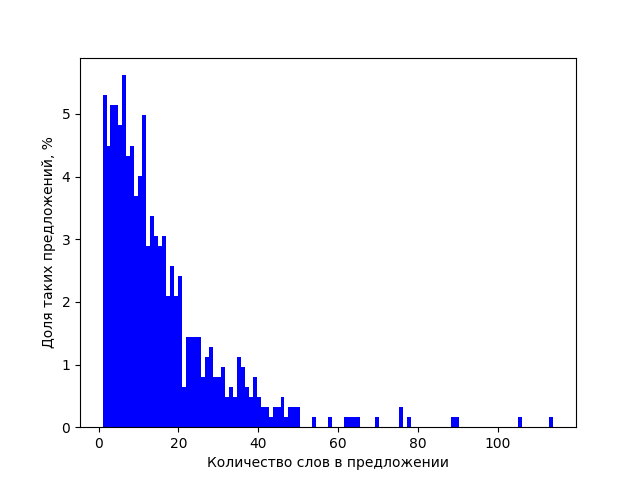
\includegraphics[width=12.564cm,height=9.449cm]{irmw2lnohyper-img1.png}
    \par}


    \bigskip


    \bigskip

    {Иллюстрация 1 показывает, что в тексте «Опера»
    эксцессы имеют единичный характер, мода (наиболее вероятный, часто
    встречающийся размер предложений) близка к среднему размеру, а потому
    текст Е. Бочоришвили нет необходимости делить на контексты прямой речи,
    речи повествователя и реплики ввода прямой речи. }

    {Основанием для вычисления среднего размера
    предложения без проведения членения текста на контексты послужил
    анализ таких произведений, в которых очевидно, что без подобного
    членения результат не может быть адекватным поставленной задаче. }

    {Для сопоставления были привлечены фрагменты
    некоторых романов 19 века, для языка повествования которых характерен
    синтагматический тип прозы. Фрагменты по размеру приблизительно равны
    тексту «Оперы», в котором содержится 26 полных страниц (для удобства
    было использовано измерение текста полными страницами). }

    {В романе Ф. М. Достоевского «Идиот» был посчитан
    средний размер }{предложений без учета контекста. }

    {\centering
    \textit{{Таблица 2}}
    \par}

    \begin{center}
    \tablehead{}
    \begin{supertabular}{|m{5.7730002cm}|m{1.6559999cm}|}
    \hline
    Слов &
    9522\\\hline
    Предложений &
    623\\\hline
    Средний размер предложения &
    15.3\\\hline
    Больше всего предложений длины &
    6\\\hline
    Таких предложений &
    35 (5.6\%)\\\hline
    Максимальная длина предложения &
    114\\\hline
    Таких предложений &
    1 (0.2\%)\\\hline
    \end{supertabular}
    \end{center}
    {}
    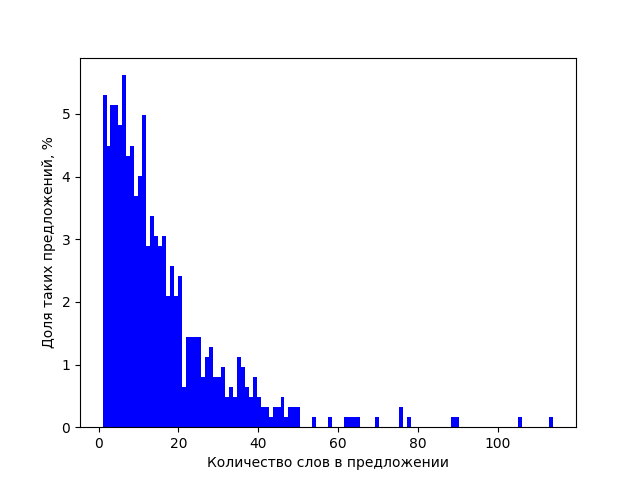
\includegraphics[width=16.933cm,height=12.7cm]{irmw2lnohyper-img2.png} 

    {Из данных таблицы и гистограммы видно, что средний
    размер предложения 15.3 достаточно далеко отстоит от наиболее
    вероятного 6, но что более значимо: встречаются предложения более чем
    из 40, 60, 80 слов, а максимальный размер равен 114. Такие экцессы не
    могут быть проигнорированы при вычислении среднего размера предложения.
    }

    {В романе И. А. Гончарова «Обломов» средний размер
    был посчитан отдельно для фрагмента, в котором преобладают реплики
    персонажей (Иллюстрация 3), и отдельно для фрагмента, по большей части
    состоящего из речи повествователя (Иллюстрация 4). Выяснилось, что в
    первом фрагменте средний размер равен 10.3, мода составила 4, что
    является несильным отклонением, эксцессы представлены несколькими
    предложениями размером от 40 до 60, и максимальный размер 61 слово.
    Второй фрагмент, преимущественно состоящий из речи повествователя,
    резко отличается от первого: средний размер возрастает до 19.3, мода 5.
    Эта разница обусловлена эксцессами: }{увеличивается
    число предложений, чей размер более 40, 60 и 80 слов, а максимальная
    длина составляет 123 слова. }

    {\centering
    \textit{{Таблица 3}}
    \par}

    \begin{center}
    \tablehead{}
    \begin{supertabular}{|m{5.7730002cm}|m{1.6559999cm}|}
    \hline
    Слов &
    8911\\\hline
    Предложений &
    861\\\hline
    Средний размер предложения &
    10.3\\\hline
    Больше всего предложений длины &
    4\\\hline
    Таких предложений &
    82 (9.5\%)\\\hline
    Максимальная длина предложения &
    61\\\hline
    Таких предложений &
    2 (0.2\%)\\\hline
    \end{supertabular}
    \end{center}
     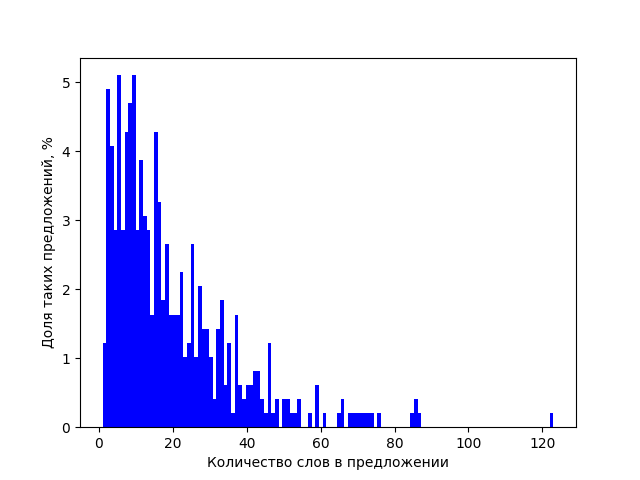
\includegraphics[width=16.933cm,height=12.7cm]{irmw2lnohyper-img3.png} 


    \bigskip


    \bigskip


    \bigskip


    \bigskip


    \bigskip


    \bigskip

    {\centering
    \textit{{Таблица 4}}
    \par}

    \begin{center}
    \tablehead{}
    \begin{supertabular}{|m{5.7730002cm}|m{1.6559999cm}|}
    \hline
    Слов &
    9472\\\hline
    Предложений &
    490\\\hline
    Средний размер предложения &
    19.3\\\hline
    Больше всего предложений длины &
    5\\\hline
    Таких предложений &
    25 (5.1\%)\\\hline
    Максимальная длина предложения &
    123\\\hline
    Таких предложений &
    1 (0.2\%)\\\hline
    \end{supertabular}
    \end{center}
     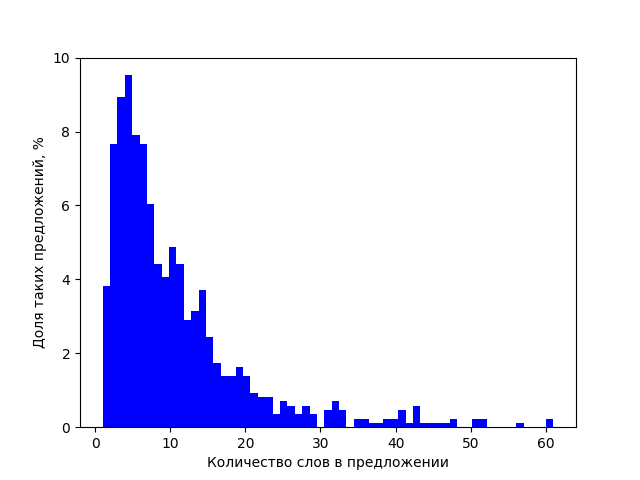
\includegraphics[width=16.933cm,height=12.7cm]{irmw2lnohyper-img4.png} 


    \bigskip


    \bigskip

    {}\textbf{{Вывод:}}{
    Так, отличительной чертой текста «Опера» является равномерность
    распределения размера предложений, отстутствие значительных эксцессов,
    и, следовательно, размытие границ между контекстами повествования
    рассказчика, речи персонажей и реплик, вводящих речь персонажей. }

    {Далее, необходимо понять, каково соотношение
    простых и сложных предложений в анализируемом тексте Е. Бочоришвили, а
    также выявить среднюю сложность текста, т. е. среднее число
    предикативных частей, составляющих сложное предложение.}

    {Методом сплошной выборки были выявлены сложные
    предложения в тексте «Опера» и посчитано их количество в отношении к
    общему числу предложений. Оказалось, что полипредикативные конструкции
    нередко }{встречаются в тексте: 30\% против 70\%,
    составляющих простые предложения.}

    {Расчет произведен по формуле: }

    {\centering
    {272 (кол-во СП) : 879 (общее число предл.) х 100 \% =
    30 \%}
    \par}

    {Как видим, сложные предложения составляют
    значительную часть текста, но при этом их размер сопоставим с размером
    простых предложений, что следует из данных Иллюстрации 1,
    свидетельствующей о крайне низком количестве эксцессов. Возникает
    вопрос о том, чем обусловлена такая сжатость полипредикативных
    конструкций. }

    {В первую очередь, посмотрим, какова картина
    распределения полипредикативных предложений, и выявим среднюю
    сложность.}


    \bigskip


    \bigskip


    \bigskip

    \begin{flushleft}
    \tablehead{}
    \begin{supertabular}{|m{3.702cm}|m{3.79cm}|}
    \hline
    \centering \textbf{{Кол-во предикативных частей в
    составе сложного предложения}} &
    \centering\arraybslash \textbf{{Количество предложений
    в тексте}}\\\hline
    \centering {2} &
    \centering\arraybslash {218}\\\hline
    \centering {3} &
    \centering\arraybslash {34}\\\hline
    \centering {4} &
    \centering\arraybslash {6}\\\hline
    \centering {5} &
    \centering\arraybslash {2}\\\hline
    \end{supertabular}
    \end{flushleft}

    \bigskip

    {Итак, наиболее часто встречающиеся предложения~---
    состоящие из 2 предикативных частей. Из таблицы видно, что роль
    эксцессов на общем фоне крайне мала. }

    {}\textbf{{Вывод:}}{
    Мы выяснили, что небольшой размер предложений обеспечивается, в
    частности, отсутствием больших полипредикативных конструкций. }

    { Далее, следует рассмотреть типичные способы
    осложнения простого предложения и частей сложного предложения, чтобы
    понять, влияют ли они (или их
    отс}{ут}{с}{т}{вие)
    на краткость предложения. }

    {В тексте встречаются самые разные способы
    осложнения предложения: как синтагматически связанные, так и
    синтагматически несвязанные. }

    {Приведем некоторые примеры.}


    \bigskip

    {\centering
    \textbf{{Синтагматически связанные средства осложнения
    предложения}}
    \par}

    {1. Обособленные определения}

    % \liststyleWWNumxv
    \begin{itemize}
    \item \begin{itemize}
    \item {И разруха пошла за войной по пятам, как
    грузинская жена, }\textit{{сопровождающая
    мужа}}{.}
    \item {Муравьи перестали ползать по нему, вверх-вниз,
    вверх-вниз, }\textit{{суетливые и
    озабоченные}}{, как мы.}
    \item {И ее понесли на руках, высоко подняв над толпой,
    и все смотрели на ее трусы, }\textit{{красные,
    собранные резинкой у колен}}{.}
    \item {И Бог,
    }\textit{{бессмертный}}{, как и
    Ленин, выслушивал молитвы и молчал.}
    \end{itemize}
    \end{itemize}
    {2. Обособленные обстоятельства}

    % \liststyleWWNumxv
    \begin{itemize}
    \item \begin{itemize}
    \item Поп подает нищим, \textit{придерживая рясу.}
    \item Нищие бросаются за подаянием, \textit{отталкивая друг друга.}
    \item И женщины расстегивали кофточки, \textit{задыхаясь от смеха.}
    \item А Жужуна сказала, что любит меня, и я опять замолчал,\textit{
    глядя в окно.}
    \end{itemize}
    \end{itemize}
    3. Уточняющие и пояснительные члены

    % \liststyleWWNumxv
    \begin{itemize}
    \item \begin{itemize}
    \item Наша директриса, \textit{Маро}, раздавала нам оплеухи, но не
    трогала его.
    \item И кажется, я не любил Ию. Тогда, \textit{в детстве}.
    \item Но мы не любили нашу бабку, \textit{ни я, ни Нанули.}
    \item Они подталкивали девушку в черном, с крестом на груди,
    \textit{жену,} наверное, \textit{или} \textit{невесту}.
    \end{itemize}
    \end{itemize}
    4. Однородные члены предложения

    % \liststyleWWNumxv
    \begin{itemize}
    \item \begin{itemize}
    \item \textit{И мясо }было, и\textit{ масло, }и у всех в доме\textit{
    пианино }было.\textit{ }
    \item Полковник \textit{пришел }наконец, \textit{разорался }и
    всех\textit{ выгнал.}
    \item Раскладывали \textit{помидоры} и вареную \textit{кукурузу}.
    \item Жители, оставшиеся в домах, \textit{своих} или \textit{чужих},
    прятались в подвалах.
    \end{itemize}
    \end{itemize}

    \bigskip

    {\centering
    \textbf{{Синтагматически не связанные средства
    осложнения предложения}}
    \par}

    {1. Вводные слова и конструкции}

    {Вводные слова и конструкции являются
    эгоцентрическими элементами, и об их встречаемости в тексте уже
    говорилось в главе 2.1. данного исследования. }

    {2. Вставные конструкции}

    % \liststyleWWNumxv
    \begin{itemize}
    \item \begin{itemize}
    \item {«Когда дерево, что росло посредине дома моего~---
    }\textit{{между печкой без газа и краном без воды,
    }}{— выбросило ягоды белые, ягоды-альбиносы».}
    \item {«Я забрался на крышу~---
    }\textit{{дерево торчало из крыши, как
    труба,}}{~--- и выше, по стволу».}
    \item «Нанули гостила в деревне у родственников отца~--- \textit{они ее
    подкармливали, я думаю,}~--- и я был один».
    \item «И не пристрелил дряхлую лошадь, \textit{нашу связь}».
    \end{itemize}
    \end{itemize}
    3. Обращения

    % \liststyleWWNumxvii
    \begin{itemize}
    \item \begin{itemize}
    \item «Я не хотел вас обидеть, \textit{батоно».}
    \item «Я должен описать тебя, \textit{Ия}, но я не нахожу в себе сил».
    \item «Здравствуйте, \textit{батоно Бог}!»
    \end{itemize}
    \end{itemize}

    \bigskip

    \textbf{Выводы:} Итак, в тексте представлены разные типы осложнения
    предложения: синтагматически связанные и не связанные. Следовательно,
    отстуствие какого-либо типа осложнения не может быть признано фактором,
    обеспечивающим краткость предложений. Данные выводы свидетельствуют о
    том, что краткость предложений обусловлена иными языковыми средствами,
    выходящими за рамки внутренней структуры цельного предложения.
    Детальный анализ способов связи предложений может стать предметом
    специального исследования. На данном этапе необходимо ограничить
    рассмотрение средств связи предложений, отобрав типичные конструкции,
    выполняющие дезинтегрирующую, актуализирующую функцию.

    В связи с поставленной задачей были рассмотрены языковые средства,
    обеспечивающие расчлененность текста, устраняющие многосложные
    полипредикативные структуры: парцеллированные конструкции и неполные
    предложения. Были рассмотрены такие явления как парцелляция и
    псевдопарцелляция. Так как для разговорного синтаксиса короткий размер
    предложений, высокая расчлененность текста, высокая роль интонации
    являются типичными, при анализе не рассматривался контекст прямой
    речи персонажей. Поиск специфических средств связи и дробления
    предложений производился на материале речи рассказчика. 

    Приведем некоторые фрагменты текста, на примере анализа которых
    покажем функционирование парцелляции и средств, оформляющих
    парцеллированные конструкции, но не позволяющих однозначно объединить
    предложения в парцеллированную конструкцию.


    \bigskip

    {\centering
    \textbf{Парцеллированные конструкции и псевдопарцелляция}
    \par}

    Для удобства работы с текстом предложения пронумерованы.

    Фрагмент 1. 

    «(1) \textcolor[rgb]{0.2,0.2,0.2}{Когда ночи вдруг стали жаркими,
    как объятия женщины. }

    \textcolor[rgb]{0.2,0.2,0.2}{(2) Когда до Тбилиси с моря долетели
    чайки. (3) Птицы грязные и крикливые. (4) Добежали беженцы. (5) Тоже
    грязные и крикливые. (6) И разруха пошла за войной по пятам, как
    грузинская жена, сопровождающая мужа. }

    \textcolor[rgb]{0.2,0.2,0.2}{(7) Когда дерево, что росло посредине
    дома моего – между печкой без газа и краном без воды, – выбросило ягоды
    белые, ягоды-альбиносы. }

    \textcolor[rgb]{0.2,0.2,0.2}{(8) Я забрался на крышу – дерево
    торчало из крыши, как труба, – и выше, по стволу. (9) Я увидел, что оно
    умирает. (10) Муравьи перестали ползать по нему, вверх-вниз,
    вверх-вниз, суетливые и озабоченные, как мы». }


    \bigskip

    \textcolor[rgb]{0.2,0.2,0.2}{В данном фрагменте усматривается
    парцелляция в следующих случаях:}

    \textcolor[rgb]{0.2,0.2,0.2}{1. Предложение 2~--- базовая структура,
    предложение 3~--- парцеллят. }

    \textcolor[rgb]{0.2,0.2,0.2}{Уточняемое слово в составе базовой
    структуры: чайки. }

    \textcolor[rgb]{0.2,0.2,0.2}{2. Предложение 4~--- базовая структура,
    предложение 5~--- парцеллят. }

    \textcolor[rgb]{0.2,0.2,0.2}{Уточняемое слово в составе базовой
    структуры: беженцы. }

    \textcolor[rgb]{0.2,0.2,0.2}{Случаи 1, 2 демонстрируют парцелляцию
    типа II.2: }\textbf{\textcolor[rgb]{0.2,0.2,0.2}{«Представленный»
    парцеллят~--- уточняющий по отношению к слову базовой структуры член
    предложения. }}

    \textbf{\textcolor[rgb]{0.2,0.2,0.2}{}}\textcolor[rgb]{0.2,0.2,0.2}{Предложения
    1, 2, 7, анафорично открывающие первые три абзаца при помощи временного
    союза «когда», имитируют придаточные предложения, основная часть
    которых, грамматически, приходится на 8 предложение. Однако
    трансформация предложений 1—8 в одно цельное предложение представляется
    неочевидной. В целях выяснения
    }\textcolor[rgb]{0.2,0.2,0.2}{возможности}\textcolor[rgb]{0.2,0.2,0.2}{
    такого объединения был проведен эксперимент по синтаксической
    трансформации. }\textcolor[rgb]{0.2,0.2,0.2}{Кроме того, для
    предоставления более полного контекста, эксперименту подверглись
    предложения 9 и 10, между которыми парцелляция не предполагается.
    }\textcolor[rgb]{0.2,0.2,0.2}{Эксперимент выполнен в форме опроса,
    участниками которого явились студенты филологического факультета СПбГУ.
    }

    \textcolor[rgb]{0.2,0.2,0.2}{}\textcolor[rgb]{0.2,0.2,0.2}{58 \%
    опрошенных представили приведенный фрагмент в виде
    }\textcolor[rgb]{0.2,0.2,0.2}{одного цельного
    предложения}\textcolor[rgb]{0.2,0.2,0.2}{. Данный факт подтверждает
    грамматическую способность предложений к синтаксической трансформации.
    }\textcolor[rgb]{0.2,0.2,0.2}{Если следовать предположению, что
    исследуемый фрагмент~--- одно цельное предложение, тогда следует выделить
    парцелляцию следующих типов: }

    \textcolor[rgb]{0.2,0.2,0.2}{1. Предложение 1, предложения 2—6,
    предложение 7~--- три придаточных предложения, начинающихся с
    подчинительного союза КОГДА.}

    \textcolor[rgb]{0.2,0.2,0.2}{Формально удовлетворяют условию I.A.3:
    }\textbf{\textcolor[rgb]{0.2,0.2,0.2}{«Непредставленный» парцеллят~---
    придаточное предложение с подчинительным союзом
    КОГДА.}}\textcolor[rgb]{0.2,0.2,0.2}{ Базовая структура: предложение
    8.}

    \textcolor[rgb]{0.2,0.2,0.2}{2. Предложение
    }\textcolor[rgb]{0.2,0.2,0.2}{6}\textcolor[rgb]{0.2,0.2,0.2}{~---
    }\textcolor[rgb]{0.2,0.2,0.2}{самостоятельное предложение, начинается с
    союза }\textcolor[rgb]{0.2,0.2,0.2}{И.}

    \textcolor[rgb]{0.2,0.2,0.2}{Ф}\textcolor[rgb]{0.2,0.2,0.2}{ормально
    удовлетворяет условию I.A.2:
    }\textbf{\textcolor[rgb]{0.2,0.2,0.2}{«Непредставленный»
    парцеллят}}\textcolor[rgb]{0.2,0.2,0.2}{~---
    }\textbf{\textcolor[rgb]{0.2,0.2,0.2}{синтаксически самостоятельное
    предложение, подключаемое к предшествующему предложению сочинительным
    союзом И.}}

    \textcolor[rgb]{0.2,0.2,0.2}{Предложения 9—10 не являются
    парцеллированной конструкцией, несмотря на возможность объединения их в
    одно цельное предложение. Связь между ними является бессоюзной,
    предложение 10 носит характер пояснения причины того, о чем говорится в
    предложении 9. Тем не менее, единственным признаком синтаксической
    несамостоятельности предложения 10 является наличие в нем местоименной
    связи с предыдущим предложением
    (}\textit{\textcolor[rgb]{0.2,0.2,0.2}{пред.9}}\textcolor[rgb]{0.2,0.2,0.2}{
    }\textbf{\textcolor[rgb]{0.2,0.2,0.2}{оно}}\textbf{\textcolor[rgb]{0.2,0.2,0.2}{
    }}\textcolor[rgb]{0.2,0.2,0.2}{—
    }\textit{\textcolor[rgb]{0.2,0.2,0.2}{пред.
    10}}\textcolor[rgb]{0.2,0.2,0.2}{
    }\textbf{\textcolor[rgb]{0.2,0.2,0.2}{по
    нему}}\textcolor[rgb]{0.2,0.2,0.2}{), что не является основанием для
    установления парцелляции какого-либо типа.}

    \textcolor[rgb]{0.2,0.2,0.2}{}\textcolor[rgb]{0.2,0.2,0.2}{Из
    рассмотренных примеров видно, что при пунктуационном оформлении данного
    фрагмента использованы средства, характерные для оформления
    парцеллированных конструкций. Более того, проведение эксперимента
    указывает на возможность осуществления синтаксической трансформации.
    Однако, по нашему мнению, возможность трансформации не указывает на
    естественность употребления конструкций такого типа в рамках одного
    предложения в контексте речи.
    }\textcolor[rgb]{0.2,0.2,0.2}{Предполагается, что в данном фрагменте
    представлена псевдопарцелляция, т. е. формальное соответствие признакам
    парцеллированных конструкций при неестественности объединения
    предложений в одно цельное предложение. }

    \textcolor[rgb]{0.2,0.2,0.2}{}\textcolor[rgb]{0.2,0.2,0.2}{На
    неоднозначность такого объединения указывают, кроме того, следующие
    данные эксперимента:}

    \textcolor[rgb]{0.2,0.2,0.2}{1. 17 \% опрошенных поставили точку
    после предложения 5.}

    \textcolor[rgb]{0.2,0.2,0.2}{2. }\textcolor[rgb]{0.2,0.2,0.2}{42 \%
    опрошенных поставили точку на месте тире в авторской версии в
    предложении 8. Такая постановка знака препинания может указывать на то,
    что соединение предыдущего фрагмента в одно предложение затрудняет
    осложнение предложения 8 вставной конструкцией. }


    \bigskip

    \textcolor[rgb]{0.2,0.2,0.2}{Как видим, установление факта
    парцелляции является сложной задачей, решение которой не всегда может
    быть однозначным. В связи с этим, опишем те явления, которые по
    формальным условиям удовлетворяют явлению парцелляции, однако не будем
    настаивать на безусловном выделении парцеллированных конструкций в
    случаях, где доказательство неочевидно. Кроме того, отметим случаи, в
    которых предложение не
    }\textcolor[rgb]{0.2,0.2,0.2}{является}\textcolor[rgb]{0.2,0.2,0.2}{
    самостоятельным, однако базовую структуру, от которой оно может быть
    отделено, выявить невозможно. }

    \textcolor[rgb]{0.2,0.2,0.2}{Фрагмент 2. }

    \textcolor[rgb]{0.2,0.2,0.2}{(1) Я задумал написать оперу, в которой
    все – мертвые. (2) И вот они являются на тот свет и ждут встречи с
    Богом. (3) И прижимают к себе вещи и вещички, которые передали с ними
    рыдающие родственники. (4) Но их встречают какие-то бюрократы, задают
    вопросы, заполняют бумаги, отбирают вещи и вещички…}

    \textcolor[rgb]{0.2,0.2,0.2}{1. Предложение 3~--- неполное
    предложение, начинается с сочинительного союза И.}

    \textcolor[rgb]{0.2,0.2,0.2}{Формально удовлетворяет условию II.1:
    }\textbf{\textcolor[rgb]{0.2,0.2,0.2}{«Представленный» парцеллят~---
    однородный по отношению к слову базовой структуры член предложения.
    }}\textcolor[rgb]{0.2,0.2,0.2}{Базовая структура~--- предложение 2.
    Однородные сказуемые: являются, ждут~--- прижимают. Дополнительное
    средство связи: сочинительный союз И.}

    \textcolor[rgb]{0.2,0.2,0.2}{2. Предложение 4~--- синтаксически
    самостоятельное предложение, начинается с сочинительного союза НО.}


    \bigskip

    \textcolor[rgb]{0.2,0.2,0.2}{Формально удовлетворяет условию I.A.2:
    }\textbf{\textcolor[rgb]{0.2,0.2,0.2}{«Непредставленный»
    п}}\textbf{{арцеллят~--- синтаксически самостоятельное
    предложение, подключаемое к предшествующему предложению сочинительным
    союз}}\textbf{{ом}}\textbf{\textit{{
    }}}\textbf{{НО.}}


    \bigskip

    {Фрагмент 3.}

    {(1) Не хоронили только в понедельник и пятницу, но
    панихиды проводились ежедневно. (2) Если, конечно, не футбол. (3) А то
    кто ж к тебе придет, если игра? (4) Или от жары. (5)
    }\textcolor[rgb]{0.2,0.2,0.2}{В такую погоду петь над покойником –
    лучше самому умереть.}

    {1. Предложение 2~--- односоставное номинативное
    предложение, начинается с условного союза ЕСЛИ.}

    {Формально удовлетворяет условию I.A.3:
    }\textbf{{«Непредставленный» парцеллят~--- придаточное
    предложение }}\textbf{{с союзом
    }}\textbf{{ЕСЛИ}}\textbf{{.
    }}{Базовая часть~--- предложение 1. }

    {2. Предложение 4~--- начинается с одиночного
    разделительного союза ИЛИ, содержит обусловленную синтаксему:
    }\textit{{от + }}{Род.п. Б.9.б.
    Внешний каузатив~--- обозначение воздействующих на субъекта явлений
    природы, различных обстоятельств, чужих действий и
    свойств.}\footnote{\textit{{ Золотова Г. А.
    }}{Синтаксический словарь. М., 2001.
    С.82}}{ }

    {Метод синтаксической трансформации не применим к
    данному предложению в виду отсутствия потенциальной структуры для
    присоединения, следовательно, предложение не является парцеллятом. Тем
    не менее, обусловленная синтаксема «каузатив», не стоящая в заголовке и
    не имеющая связи с каким-либо членом предложения, а также начальный
    союз ИЛИ указывают на несамостоятельность и неполноту предложения. }


    \bigskip

    {Фрагмент 4.}

    {(1) Это лето пришло без весны. (2) И без запаха
    фиалок. (3) Каждую весну на всех углах улиц продавали фиолетовые
    фиалки. (4) За пять копеек продавали весну. (5) Сейчас торговали
    трупами и местами захоронений. (6) Обменивали
    }{пленных. (7) Брали пленных впрок. (8) И пули купить
    было проще, чем цветы.}

    {1. Предложение 2~--- начинается с сочинительного
    союза И, содержит свободную синтаксему, но в функции компонента
    предложения: }\textit{{Без }}{+ Род.
    п.}{ А.II. 4.3. В качестве вторичного предиката в
    осложненных моделях.}\footnote{{
    }\textit{{Золотова Г. А.
    }}{Синтаксический словарь. М., 2001. С.39}}

    {Формально соответствует }{условию
    II.1}{:
    }\textbf{\textcolor[rgb]{0.2,0.2,0.2}{«Представленный» парцеллят~---
    однородный по отношению к слову базовой структуры член предложения.
    }}\textcolor[rgb]{0.2,0.2,0.2}{Базовая структура~--- предложение 1.
    Однородные члены предложения: весны~--- запаха фиалок.}

    \textcolor[rgb]{0.2,0.2,0.2}{2. Предложения 6, 7~--- неполные
    предложения.}

    {Формально
    }{удовлетворяют}{
    }{условию II.1}{:
    }\textbf{\textcolor[rgb]{0.2,0.2,0.2}{«Представленный» парцеллят~---
    однородный по отношению к слову базовой структуры член предложения.
    }}\textcolor[rgb]{0.2,0.2,0.2}{Базовая структура~--- предложение 5.
    Однородные члены предложения: торговали~--- обменивали; брали.}

    \textcolor[rgb]{0.2,0.2,0.2}{Ф}\textcolor[rgb]{0.2,0.2,0.2}{рагмент
    5}

    «(1) Она закрывала их, чтобы не видеть, как я одеваюсь. (2) Как я
    ухожу. (3) Свешиваюсь с балкона и прыгаю наземь».

    Предложения 2, 3~--- неполные предложения. 

    {Формально
    }{удовлетворяют}{
    }{условию }{II.2}{:
    }\textbf{\textcolor[rgb]{0.2,0.2,0.2}{«Представленный» парцеллят~---
    однородный по отношению к слову базовой структуры член предложения.
    }}\textcolor[rgb]{0.2,0.2,0.2}{Базовая структура~--- предложение
    }\textcolor[rgb]{0.2,0.2,0.2}{1}\textcolor[rgb]{0.2,0.2,0.2}{.
    Однородные члены предложения: }\textcolor[rgb]{0.2,0.2,0.2}{одеваюсь~---
    ухожу; свешиваюсь, прыгаю.}

    \textcolor[rgb]{0.2,0.2,0.2}{Фрагмент 5}

    {\color[rgb]{0.2,0.2,0.2}
    «(1) Трусы у всех были из красного шелка. (2) Советский флаг, а не
    трусы».}

    {\color[rgb]{0.2,0.2,0.2}
    Предложение 2~--- односоставное номинативное предложение. }

    {\color[rgb]{0.2,0.2,0.2}
    Формально удовлетворяет условию II.2: \textbf{«Представленный»
    парцеллят~--- уточняющий по отношению к слову базовой структуры член
    предложения. }Базовая структура: предложение 1. }


    \bigskip

    {\color[rgb]{0.2,0.2,0.2}
    Фрагмент 6}

    {\color[rgb]{0.2,0.2,0.2}
    «(1) И когда это случилось, в церковном дворе, поп был виновен, как
    ни крути. (2) Это он попросил Эстате: “Сделай что-нибудь, нельзя, чтобы
    ворон сидел на церковном кресте”. (3) Потому что для Эстате что вороны,
    что чайки. (4) И теперь Эстате мучит раскаяние». }

    {\color[rgb]{0.2,0.2,0.2}
    Предложение 3~--- начинается с подчинительного союза ПОТОМУ ЧТО. }

    {\color[rgb]{0.2,0.2,0.2}
    Формально удовлетворяет условию I.А.3: \textbf{«Непредставленный»
    парцеллят~--- придаточное предложение с союзом ПОТОМУ ЧТО.} }

    {\color[rgb]{0.2,0.2,0.2}
    Не является парцеллятом в силу невозможности экспериментальной
    трансформации. Потенциальная базовая структура (предложение 1) не
    является семантически достаточной для присоединения предложения 3. }

    {\color[rgb]{0.2,0.2,0.2}
    Фрагмент 7}

    {\color[rgb]{0.2,0.2,0.2}
    «(1) Эстате будит меня по воскресеньям, и мы идем в церковь. (2)
    Напрямик, через кладбище для знаменитых людей».}

    {\color[rgb]{0.2,0.2,0.2}
    Предложение 2~--- распространенный зависимый член предложения с
    обстоятельственым значением, состоящий из наречия и предложно-падежной
    формы. }

    {\color[rgb]{0.2,0.2,0.2}
    Формально удовлетворяет условию I.B.1:
    \textbf{«}\textbf{Нерпредставленный» парцеллят~--- зависимый член
    предложения, факультативно распространяющий }\textbf{какое-либо слово
    или всю предикативную основу базовой структуры. }Базовая структура:
    предложение 1.}

    {\color[rgb]{0.2,0.2,0.2}
    Фрагмент 8}

    {\color[rgb]{0.2,0.2,0.2}
    « (1) Старики надевали галоши. (2) Черные и блестящие, как
    правительственные машины».}

    {\color[rgb]{0.2,0.2,0.2}
    Предложение 2~--- не является самостоятельным предложением. Состоит из
    согласованного определения и именной сравнительной конструкции.}

    {\color[rgb]{0.2,0.2,0.2}
    Формально удовлетворяет условию I.B.1:
    \textbf{«}\textbf{Непредставленный» парцеллят~--- зависимый член
    предложения, факультативно распространяющий какое-либо слово или всю
    предикативную основу базовой структуры.}}

    {\color[rgb]{0.2,0.2,0.2}
    Базовая структура: предложение 1. }

    {\bfseries\color[rgb]{0.2,0.2,0.2}
    Выводы: \textmd{Для текста «Опера» характерны следующие
    синтаксические особенности:}}

    {\bfseries\color[rgb]{0.2,0.2,0.2}
    \textmd{1. Использование парцеллированных конструкций;}}

    {\bfseries\color[rgb]{0.2,0.2,0.2}
    \textmd{2. Псевдопарцелляция, т. е. организация предложений при
    помощи признаков парцеллированных конструкций }\textmd{без возможности
    объединения таких предложений в одно цельное предложение.}}

    {\bfseries\color[rgb]{0.2,0.2,0.2}
    \textmd{}Парцеллированные конструкции\textmd{ }\textmd{реализуются
    через отделение от базовой структуры парцеллятов следующих
    типов}\textmd{:}}

    {\bfseries\color[rgb]{0.2,0.2,0.2}
    \textmd{}\textmd{1. Парцелляты, не представленные ни одним членом
    предложения в составе базовой структуры. Парцелляты такого типа могут
    являться следующими единицами:}}

    {\bfseries\color[rgb]{0.2,0.2,0.2}
    \textmd{1.1. Зависимый член предложения, факультативно
    распространяющий базовую структуру.}}

    {\bfseries\color[rgb]{0.2,0.2,0.2}
    \textmd{1.2. }\textmd{Синтаксически самостоятельное предложение,
    подключаемое к предшествующему предложению сочинительными союзами.}}

    {\bfseries\color[rgb]{0.2,0.2,0.2}
    \textmd{1.3. Придаточное предложение с подчинительным союзом.}}

    {\bfseries\color[rgb]{0.2,0.2,0.2}
    \textmd{2. Парцелляты, представленные в базовой структуре каким-либо
    членом предложения. Парцелляты могут быть связаны с базовой структурой
    следующими способами:}}

    {\bfseries\color[rgb]{0.2,0.2,0.2}
    \textmd{2.1. Однородный по отношению к слову базовой}}

    {\bfseries\color[rgb]{0.2,0.2,0.2}
    \textmd{конструкции член предложения;}}

    {\bfseries\color[rgb]{0.2,0.2,0.2}
    \textmd{2.2. Уточняющий по отношению к слову базовой}}

    {\bfseries\color[rgb]{0.2,0.2,0.2}
    \textmd{структуры член предложения.}}

    {\bfseries\color[rgb]{0.2,0.2,0.2}
    \textmd{}Псевдопарцелляция\textmd{ реализуется на основе:}}

    {\bfseries\color[rgb]{0.2,0.2,0.2}
    \textmd{1. }\textmd{Полных двусоставных п}\textmd{редложений,
    начинающихся с сочинительных или подчинительных союзов;}}

    {\bfseries\color[rgb]{0.2,0.2,0.2}
    \textmd{2. }\textmd{Зависимых членов предложения, }\textmd{не
    имеющих потенциальной базовой структуры, }\textmd{но оформленных как
    самостоятельная коммуникативная единица. }}


    \bigskip

    \clearpage{\centering\bfseries\color[rgb]{0.2,0.2,0.2}
    Ввод персонажей, указание на время
    \par}

    {\color[rgb]{0.2,0.2,0.2}
    \textcolor[rgb]{0.0,0.0,0.039215688}{Как было отмечено в Главе 1.1,
    в тексте стенограммы содержится точное указание на время, в которое
    происходит событие, а также на авторов реплик.}}

    {\color[rgb]{0.2,0.2,0.2}
    \textcolor[rgb]{0.0,0.0,0.039215688}{В художественном тексте Е.
    Бочоришвили данные особенности стенограммы находят специфическое
    отражение. }}

    {\centering\bfseries\color[rgb]{0.2,0.2,0.2}
    \textcolor[rgb]{0.0,0.0,0.039215688}{Ввод персонажей }
    \par}

    {\color[rgb]{0.2,0.2,0.2}
    \textcolor[rgb]{0.0,0.0,0.039215688}{}\textcolor[rgb]{0.0,0.0,0.039215688}{Первая
    глава текста}\textcolor[rgb]{0.0,0.0,0.039215688}{
    }\textcolor[rgb]{0.0,0.0,0.039215688}{представляет
    собой}\textcolor[rgb]{0.0,0.0,0.039215688}{
    }\textcolor[rgb]{0.0,0.0,0.039215688}{оформленный как текст драмы
    }\textcolor[rgb]{0.0,0.0,0.039215688}{диалог двух персонажей, реплики
    которых не авторизованы. }\textcolor[rgb]{0.0,0.0,0.039215688}{Вторая
    глава, }\textcolor[rgb]{0.0,0.0,0.039215688}{где диалог сменяется речью
    перволичного повествователя, не содержит прямого пояснения того, в
    каком контексте происходил диалог предыдущей главы и кто его
    осуществляет.}\textcolor[rgb]{0.0,0.0,0.039215688}{
    }\textcolor[rgb]{0.0,0.0,0.039215688}{Первое
    }\textcolor[rgb]{0.0,0.0,0.039215688}{косвенное}\textcolor[rgb]{0.0,0.0,0.039215688}{
    указание содержится }\textcolor[rgb]{0.0,0.0,0.039215688}{лишь
    }\textcolor[rgb]{0.0,0.0,0.039215688}{в одном абзаце второй
    гл}\textcolor[rgb]{0.0,0.0,0.039215688}{а}\textcolor[rgb]{0.0,0.0,0.039215688}{вы:}}

    {\color[rgb]{0.2,0.2,0.2}
    «Я задумал написать оперу, в которой все – мертвые. И вот они
    являются на тот свет и ждут встречи с Богом. И прижимают к себе вещи и
    вещички, которые передали с ними рыдающие родственники. \textbf{Но их
    встречают какие-то бюрократы, задают вопросы, заполняют бумаги,}
    отбирают вещи и вещички…».}

    {\color[rgb]{0.2,0.2,0.2}
    Можно предположить, что участники диалога~--- герои «оперы», которую
    задумал написать рассказчик. }

    {\color[rgb]{0.2,0.2,0.2}
    Продолжается «прерванный» повествованием диалог в пятой главе , где
    снова нет указания на авторов реплик. Сопоставляя речь одного из
    участников диалога с прямой речью, которую мы встретим в конце седьмой
    главы в рамках повествования рассказчика, можно понять, что описываемый
    в седьмой главе погибший «старик» и есть один из авторов реплик
    диалогов (главы 1, 5), а именно~--- допрашиваемый. }

    {\color[rgb]{0.2,0.2,0.2}
    Глава 5:}

    {\color[rgb]{0.2,0.2,0.2}
    «– Напоминаю вам: вы не имеете права задавать вопросы. \textbf{У вас
    отрезали мизинец}, потому что не могли снять с него перстень. А портрет
    \textbf{вашей жены }\textbf{Маргариты}, что был при вас, не тронули.}

    {\color[rgb]{0.2,0.2,0.2}
    \textless{}...\textgreater{}}

    {\color[rgb]{0.2,0.2,0.2}
    – \textbf{Маргарита}, любовь моя. Я хочу видеть Маргариту».}

    {\color[rgb]{0.2,0.2,0.2}
    Глава 7:}

    {\color[rgb]{0.2,0.2,0.2}
    «Не дали тебе умереть по-человечески, – причитала она, – на старика
    руку подняли! Будь они прокляты, фашисты это, а не люди!
    \textbf{Маргарита}, куда ты смотрела? Из-за \textbf{перстня} какого-то
    человека убить?...»}

    {\color[rgb]{0.2,0.2,0.2}
    Так, одним из методов ввода персонажа является вставка в текст его
    речи в контексте диалога, рамкой (но не финальной границей) которого
    является глава. Определяющей чертой оформления такого диалога является
    отсутствие указания на имя, статус или иные характеристики участников
    диалога. Установление личности говорящего осуществляется как
    «узнавание» через косвенные указания, содержащиеся в речи рассказчика
    и прямой речи других персонажей. }

    {\color[rgb]{0.2,0.2,0.2}
    Другим способом ввода персонажа является неподготовленное
    описанием личности употребление ранее не встречавшегося имени, за
    которым также не следует никакого прямого указания на то, кем является
    упомянутый персонаж. Он беспрепятственно фигурирует как участник
    описываемых событий, а идентификация происходит постепенно: через
    накопление информации о поступках персонажа, через его речь, а также
    комментарии рассказчика. Приведем примеры ввода персонажей, при которых
    отсутствует какое-либо общее указание на их роль в рамках мира
    повествования: }

    {\color[rgb]{0.2,0.2,0.2}
    1. «Я больше не боялся землетрясений. Я однажды танцевал, когда
    трясло. Эстате снимал туфлю и бил тараканов каблуком. И ждал: кто
    следующий, а?»}

    {\color[rgb]{0.2,0.2,0.2}
    2. «Жужуна опять пополнела, и ее глаза ушли вглубь, как амбразуры.
    Она закрывала их, чтобы не видеть, как я одеваюсь». }

    {\color[rgb]{0.2,0.2,0.2}
    3. «А Аннушка сказала: “Спасибо тебе, Господи, за то, что на свете
    есть красота”.»}


    \bigskip

    {\color[rgb]{0.2,0.2,0.2}
    Такое употребление имен характерно для речевой ситуации, при которой
    участники диалога обладают «частной апперцепционной
    базой»\footnote{\textit{Земская Е. Н. Китайгородская М. В.
    }\textit{Ширяев Е. Н. }Русская разговорная речь. Общие вопросы.
    Словообразование. Синтаксис/Конситуативные высказывания// М., 1981.
    С.195}, знанием и опытом конкретных партнеров коммуникации,
    позволяющим не давать поясняющий комментарий к употребленному имени.
    Сходное употребление имен мы встречаем и в тексте стенограммы, где
    реплике предшествует имя, но, как правило, отсутствует поясняющий
    комментарий о том, кем является говорящий. В некоторых случаях, однако,
    помимо имени, встречается краткая характеристика говорящего, например,
    если его роль является значимой с организационной точки зрения:
    «Председательствующий тов. Хрущев».\footnote{См.: Пример 2 в
    «Приложении» к данной работе.} }

    {\color[rgb]{0.2,0.2,0.2}
    Еще одним способом ввода персонажа является поименование и краткий
    постпозитивный комментарий, который носит характер попутного уточнения.
    Приведем примеры:}

    {\color[rgb]{0.2,0.2,0.2}
    1. «И кто-то все-таки попал под колеса. И Васо, \textbf{соседа
    моего}, затаскали по кабинетам полиции. А у Васо ноги опухали. Он всю
    жизнь провел в шлепанцах. Он троллейбус водил не обувшись. И теперь он
    ходил на допросы в ботинках и плакал легко».}

    {\color[rgb]{0.2,0.2,0.2}
    2. «А жилец с восьмого этажа, \textbf{художник}, поймал голубей и
    выкрасил их в розовый цвет».}

    {\color[rgb]{0.2,0.2,0.2}
    \textcolor[rgb]{0.0,0.0,0.039215688}{}\textcolor[rgb]{0.0,0.0,0.039215688}{3.
    «}Маленькая Анна, \textbf{внучка Аннушки}, затягивает ленты на ее
    спине».}

    {\color[rgb]{0.2,0.2,0.2}
    Таким образом, в тексте присутствует три типа ввода персонажей: }

    {\color[rgb]{0.2,0.2,0.2}
    1. Приведение речи персонажей в форме диалога без авторизации;}

    {\color[rgb]{0.2,0.2,0.2}
    2. Называние персонажа по имени без поясняющего комментария;}

    {\color[rgb]{0.2,0.2,0.2}
    3. Называние персонажа с кратким поясняющим комментарием.}

    {\color[rgb]{0.2,0.2,0.2}
    Подобные способы ввода персонажей позволяют имитировать
    безоценочность в фиксации речи и событий, предоставляя читателю
    возможность самостоятельно сконструировать личность героев. Уход от
    последовательного описания характера, внешности, статуса и других черт
    героев повествования позволяет имитировать объективность в передаче
    событий и сконцентрировать внимание на них, а не на точке зрения
    рассказчика, его оценке персонажей. }

    {\centering\bfseries\color[rgb]{0.2,0.2,0.2}
    Время событий. Условность жанра
    \par}

    {\color[rgb]{0.2,0.2,0.2}
    В стенограмме присутствует указание на дату события (см.: Пример
    1, Пример 2 в «Приложении»). В тексте «Опера» время события
    обозначается иным способом. Вторая глава, в которой появляется голос
    рассказчика, начинается с обозначения времени описываемых событий, о
    чем свидетельствует временной союз «когда», открывающий три первых
    абзаца. }

    {\color[rgb]{0.2,0.2,0.2}
    «\textbf{Когда} ночи вдруг стали жаркими, как объятия женщины.}

    {\color[rgb]{0.2,0.2,0.2}
    \textbf{Когда} до Тбилиси с моря долетели чайки. Птицы грязные и
    крикливые. Добежали беженцы. Тоже грязные и крикливые. И разруха пошла
    за войной по пятам, как грузинская жена, сопровождающая мужа.}

    {\color[rgb]{0.2,0.2,0.2}
    \textbf{Когда} дерево, что росло посредине дома моего – между печкой
    без газа и краном без воды, – выбросило ягоды белые, ягоды-альбиносы».}

    {\color[rgb]{0.2,0.2,0.2}
    Как и в тексте стенограммы, обозначение времени занимает выделенное
    положение по отношению к основному тексту. Однако реальная дата в
    тексте «Опера» заменяется использованием временного союза, после
    которого следует описание обстановки и важных для повествователя черт,
    художественно характеризующих время. Именно данной задачей
    художественной трансформации реальной черты оформления стенограммы
    обусловлено выделение приведенных начальных предложений 2 главы в
    отдельные самостоятельные абзацы. Так, черта стенограммы художественно
    трансформируется автором, обнажая условность жанра. }

  \clearpage{\centering\bfseries
  \hypertarget{5xjgokphfqw9}{}Приложение
  \par}

  {\bfseries
  \hypertarget{vt49pj7hzs12}{}Примеры стенограмм  }

  Пример №1. 

  Фрагмент расшифрованного текста стенограммы. Красным цветом в тексте
  выделены комментарии стенографа, представляющие собой указание на
  автора речи и попутные замечания о реакции аудитории. Жирным шрифтом
  отмечено указание на время проведения заседания и тему заседания.


  \bigskip


  \bigskip

  «\textbf{{Заседание 4 декабря 1936 года}}

  \textbf{{Утверждение проекта Конституции}}\footnote{
  Вопросы истории, 1995, № 1. Политический архив XX в. Фрагменты
  стенограммы декабрьского пленума ЦК ВКП(б) 1936 года.\par Ссылка на
  электронный ресурс:
  http://old.memo.ru/history/1937/dec\_1936/index.htm}

  \textcolor[rgb]{0.70980394,0.1764706,0.13725491}{Молотов.}{
  Товарищи, разрешите объявить заседание пленума открытым. В повестке дня
  два вопроса. Первый вопрос~--- об окончательном тексте Конституции и
  второй вопрос~--- доклад т. Ежова о троцкистских и правых антисоветских
  организациях. Есть ли другие предложения по поводу повестки дня
  пленума? (}\textcolor[rgb]{0.70980394,0.1764706,0.13725491}{Голоса с
  мест.}{ Утвердить). По первому вопросу слово имеет т.
  Сталин.}

  \textcolor[rgb]{0.70980394,0.1764706,0.13725491}{Сталин.}{
  Все читали проект Конституции?}

  \textcolor[rgb]{0.70980394,0.1764706,0.13725491}{Молотов.}{
  Все присутствовали на вчерашнем заседании комиссии, значит, можно
  проект не зачитывать. Есть какие-либо замечания?}

  \textcolor[rgb]{0.70980394,0.1764706,0.13725491}{Каминский.}{
  У меня следующее замечание. Во второй главе «Государственное
  устройство» в пункте «с» сказано: «Установление основных начал в
  области просвещения и здравоохранения». В связи с созданием союзного
  Наркомздрава речь будет итти не только об установлении основных начал в
  области здравоохранения, но и о руководстве эпидемической борьбой, о
  целом ряде мероприятий, о борьбе с чумой, об оборонных мероприятиях и
  т. д. Исходя из этого, я вношу следующую поправку. Сказать так:
  «Установление основных начал в области просвещения и руководство
  системой здравоохранения». Я это мотивирую тем, что в пункте «л»
  говорится о том, что все наркоматы имеют основание для руководства,
  чего не сказано про учреждения здравоохранения. В таком случае Народный
  комиссар здравоохранения не будет иметь право решать целого ряда
  вопросов. В области здравоохранения сейчас меньше всего идет речь об
  установлении основных начал, а больше дело касается конкретных
  мероприятий по управлению, по организации бактериологии, организации
  курортного дела и т. д.}

  \textcolor[rgb]{0.70980394,0.1764706,0.13725491}{Сталин.}{
  Видите, Конституция мешает им лучше работать. Чепуха какая!}

  \textcolor[rgb]{0.70980394,0.1764706,0.13725491}{Молотов.}{
  Разрешите голосовать поправку.
  (}\textcolor[rgb]{0.70980394,0.1764706,0.13725491}{Голоса с
  мест.}{ Не стоит голосовать.)}

  \textcolor[rgb]{0.70980394,0.1764706,0.13725491}{Каминский.}{
  Тогда разрешите сказать о второй поправке.
  (}\textcolor[rgb]{0.70980394,0.1764706,0.13725491}{Каганович.}{
  Учтите опыт первой.
  }\textcolor[rgb]{0.70980394,0.1764706,0.13725491}{Общий
  смех.}{) Учту, учту. Я вношу поправку к статье 76-ой,
  где надо сказать: предприятия и учреждения, потому что не все можно
  назвать предприятием.
  (}\textcolor[rgb]{0.70980394,0.1764706,0.13725491}{Микоян.}{Почему
  нельзя назвать?) По-моему, Институт охраны материнства и младенчества
  никак нельзя назвать предприятием.
  (}\textcolor[rgb]{0.70980394,0.1764706,0.13725491}{Микоян.}{
  А почему нельзя?) Это учреждение, а не предприятие. В самой Конституции
  устанавливается разница между предприятиями и учреждениями.}

  \textcolor[rgb]{0.70980394,0.1764706,0.13725491}{Уншлихт.}{
  У меня есть поправка. В главе третьей, в статье 49 говорится о том, что
  производится всенародный опрос (референдум). По-моему, вместо
  «всенародный опрос» нужно сказать «всенародное голосование».}

  \textcolor[rgb]{0.70980394,0.1764706,0.13725491}{Сталин.}{
  Голосование бывает тогда, когда выбирают. Опрос лучше.
  (}\textcolor[rgb]{0.70980394,0.1764706,0.13725491}{Любченко.}{
  Правильно, это лучше. Референдум это и есть всенародный
  опрос.}\textcolor[rgb]{0.70980394,0.1764706,0.13725491}{
  Ворошилов.}{ Референдум выявляет, определяет
  настроения.)}

  \textcolor[rgb]{0.70980394,0.1764706,0.13725491}{Молотов.}{
  Следовательно, поправка отклоняется.}

  \textcolor[rgb]{0.70980394,0.1764706,0.13725491}{Уншлихт.}{
  Следующая поправка к главе IV к статье 58, где устанавливаются нормы
  представительства конституций союзных республик. Конституции
  принимаются республиканскими съездами. А в статье 60 говорится, что
  Верховный Совет принимает конституцию республик и вносит свои
  изменения. Таким образом выходит, что один раз принимает конституцию
  съезд, а другой раз...
  (}\textcolor[rgb]{0.70980394,0.1764706,0.13725491}{Каганович.}{
  Съездов больше не будет.) А республиканские?
  (}\textcolor[rgb]{0.70980394,0.1764706,0.13725491}{Каганович.}{
  То же самое, их не будет.) Последняя статья говорит об этом
  определенно.
  (}\textcolor[rgb]{0.70980394,0.1764706,0.13725491}{Любченко.}{
  А если он захочет принять, нельзя?) Можно принять, но тут говорится,
  что после того, как выбирается Верховный Совет, тут же принимает
  конституцию.
  (}\textcolor[rgb]{0.70980394,0.1764706,0.13725491}{Движение в зале.
  Реплики.}{)».}{\textsuperscript{1}}


  \bigskip

  2. Пример №2. Фрагмент расшифрованного текста стенограммы.


  \bigskip

  «\textbf{{Неправленная стенограмма июльского (1964 г.)
  Пленума ЦК КПСС.}}\footnote{ Артизов А. Н. Сигачев Ю. В. Россия. XX
  век// Опубликовано в альманахе по: Никита Хрущев. 1964: Стенограммы
  пленума ЦК КПСС и другие документы. М.: МФД: Материк, 2007. С. 52–61.}

  \textbf{{11 июля 1964 г.}}

  \textbf{{Заседание первое}}

  \textbf{{Утреннее}}

  \textcolor[rgb]{0.77254903,0.0,0.043137256}{Председательствующий тов.
  ХРУЩЕВ.}{ Президиум ЦК, товарищи, решил собрать Пленум
  Центрального Комитета исключительно по вопросам сессии. Других никаких
  вопросов не }{подготовили, но мы считали, что
  следовало бы обменяться по вопросам, которые мы подготовили для
  сессии.}

  {Прежде всего, о присутствующих. Из 169 членов
  Центрального Комитета на Пленуме присутствует 152, из 149 кандидатов~---
  131, из 63 членов Центральной Ревизионной Комиссии~--- 61. Таким образом,
  разрешите Пленум объявить открытым.}

  {Прежде всего, мы раньше условились, что надо выдвинуть
  Председателя Президиума Верховного Совета СССР с тем, чтобы освободить
  товарища Брежнева. Есть такое предложение: освободить товарища Брежнева
  от обязанностей Председателя Президиума Верховного Совета. Вместо
  товарища Брежнева выдвигается кандидатура товарища Микояна Анастаса
  Ивановича. Я думаю, что вы все-таки слышали о нем.
  (}\textcolor[rgb]{0.77254903,0.0,0.043137256}{Смех}{).}

  {Кто дает ему отлуп, как сказал товарищ Шолохов,
  вернее, не Шолохов, а как сказал Щукарь. Когда он давал отлуп, Анастас
  Иванович? Вот экзамен. Не знает. За это тебе, может быть, отлуп дать?}

  \textcolor[rgb]{0.77254903,0.0,0.043137256}{ШОЛОХОВ.}{
  Может быть, нашему дорогому Анастасу Ивановичу...}

  {Председательствующий тов. ХРУЩЕВ. Как дед Щукарь?}

  {Я вижу, что у Пленума игривое настроение. Это, видимо,
  хороший признак, и по существу никто не возражает?}

  \textcolor[rgb]{0.77254903,0.0,0.043137256}{ГОЛОСА.}{
  Нет.
  (}\textcolor[rgb]{0.77254903,0.0,0.043137256}{Аплодисменты}{).}

  {Председательствующий тов. ХРУЩЕВ. Почему он
  аплодирует? (}\textcolor[rgb]{0.77254903,0.0,0.043137256}{Обращается к
  товарищу Брежневу}{). Это рады, чтобы Вас освободить.
  Нельзя же назначить, не освободивши. Это обрадовались люди, что Вас
  освободили.}

  \textcolor[rgb]{0.77254903,0.0,0.043137256}{БРЕЖНЕВ.}{
  Не думаю. Это они хорошо провожают.}

  \textcolor[rgb]{0.77254903,0.0,0.043137256}{Председательствующий тов.
  ХРУЩЕВ.}{ Думаю, что никто не требует голосования,
  поэтому будем считать, что одни аплодируют~--- поддерживают, другие
  аплодируют~--- провожают. Так?}

  {Я думаю, что это будет хорошо, потому что сейчас
  значение Президиума Верховного Совета надо поднимать и придавать ему
  еще большее значение. Вот Конституцию разработали. Нам вообще надо,
  если нас китайцы критикуют за то, что их в Программе исключили, не
  записали о диктатуре пролетариата,~--- то нам сейчас не завинчивать гайки
  надо, а надо показать силу социалистической демократии. У нас это есть.
  Вы смотрите, мы когда-то как жили. В первые годы революции черт-те чего
  у нас в стране не было, а мы жили, мы победили. У нас оппозиции были,
  были социал-революционеры, были анархисты, были меньшевики, черт знает
  сколько их было, сейчас не подсчитаешь, и мы выжили. Теперь, когда мощь
  в народе, }{когда мы сильны, а экономика~--- это
  доказательство правильности марксистско-ленинского учения, сейчас нужно
  создать условия.}

  {При демократии, конечно, может быть всякое. Раз
  демократия, то и руководство может быть подвергнуто критике. И это надо
  понимать. Без критики нет демократии. Тогда раз сказал, значит, враг
  народа~--- тащи его в каталажку с судом или без суда. От этого мы ушли,
  это мы осудили. Я бы сказал, если это не позорное, то неприятное
  прошлое~--- то, что было. Неприятное потому, что ничем не вызывалось. Мы
  антидемократические методы побороли со всеми трудностями и разбили
  врагов, оппозицию, имели монолитность в народе, который поддерживал
  нашу партию, а сейчас, я так понимаю, не все мы единого мнения, сейчас
  у нас по нарастающей развивается этот процесс. Поэтому, чтобы было
  более демократично~--- надо устранить препятствия: освободить одного и
  выдвинуть другого. Анастас доволен, доволен
  (}\textcolor[rgb]{0.77254903,0.0,0.043137256}{смех}{).
  Правильно я сказал?}

  \textcolor[rgb]{0.77254903,0.0,0.043137256}{БРЕЖНЕВ.}{
  Насчет Анастаса?}

  \textcolor[rgb]{0.77254903,0.0,0.043137256}{ХРУЩЕВ.}{
  Да.
  (}\textcolor[rgb]{0.77254903,0.0,0.043137256}{Смех}{).}

  {Мы запишем о том, для чего мы делаем, чтобы т. Брежнев
  в ЦК работал, выполнял свои обязанности секретаря ЦК. Вот, собственно
  говоря, по этим вопросам.}

  {Теперь повестка дня сессии. Мы так формулируем этот
  вопрос: о мерах по выполнению Программы КПСС в области повышения
  благосостояния народа. А потом разбивается по подпунктам. В чем это
  выражается?}

  {а) О пенсиях и пособиях колхозникам.}

  {б) О повышении заработной платы работникам
  просвещения, здравоохранения, жилищно-коммунального хозяйства,
  торговли, общественного питания и других отраслей народного хозяйства.
  Вот один вопрос.}

  {Меня докладчиком утвердили. Я думаю, что вы не
  заставите меня, чтобы я доклад делал, а я готов. Я знаю, что они не
  захотят, поэтому я проявил храбрость.
  (}\textcolor[rgb]{0.77254903,0.0,0.043137256}{Смех}{).
  Я, собственно, не готов к докладу на Пленуме, думаю, что члены ЦК и не
  требуют этого».}
\end{document}
